In this chapter we move away from the ScatterNet ideas from the previous 
chapters and instead look at using the wavelet domain as a new space in which to
learn. With ScatterNets, complex wavelets are used to scatter the energy into
different channels (corresponding to the different wavelet subbands), before the
complex modulus demodulates the signal to low frequencies. These channels can
then be mixed before scattering again (as we saw in the learnable scatternet),
but the progressive stages all result in a steady demodulation of signal energy
towards zero frequency. 

In this chapter we introduce the \emph{wavelet gain layer}
which starts in a similar fashion to the ScatterNet -- by taking the $\DTCWT$ of
a multi-channel input. Next, instead of taking a complex modulus, we learn a 
complex gain for each subband in each input channel. A single value here can 
amplify or attenuate all the energy in one part of the frequency plane. Then, 
while still in the wavelet domain, we mix the different input channels by subband (e.g.
all the $15\degs$ wavelet coefficients are mixed together, but the $15\degs$ and
$45\degs$ coefficients are not). We can then return to the pixel
domain with the inverse wavelet transform. 

We also briefly explore the possibility of doing nonlinearities in the wavelet
domain. The goal being to ultimately connect multiple wavelet gain layers
together with nonlinearities before returning to the pixel domain. 

The proposed wavelet gain layer can then be used in conjunction with regular
convolutional layers, with a network moving into the wavelet or pixel space and
learning filters in one that would be difficult to learn in the other.

Our experiments so far have shown some promise. We are able to learn complex
wavelet gains and a network with one or two gain layers shows small improvements. 
We have also found that the ReLU works well in the wavelet domain as a
nonlinearity.

However, replacing a convolutional layer with a gain layer degrades performance
by a small amount.

% Additionally, we have not been successful in finding a nonlinearity that works
% well in the wavelet domain. 

\section{Related Work}\label{sec:ch6:related} 
\subsection{Wavelets as a Front End}
Fujieda et.\ al.\ use a DWT in combination with a
CNN to do texture classification and image annotation 
\cite{fujieda_wavelet_2017, fujieda_wavelet_2018}. In particular, they take a
multiscale wavelet transform of the input image, combine the actviations at each
scale independently with learned weights, and feed these back into the network
where the activation resolution size matches the subband resolution. The
architecture block diagram is shown in \autoref{fig:ch6:fujieda}, taken from the
original paper.  This work found that their dubbed `Wavelet-CNN' could
outperform competetive non wavelet based CNNs on both texture classification and
image annotation.

\begin{figure}[bt]
  \centering
  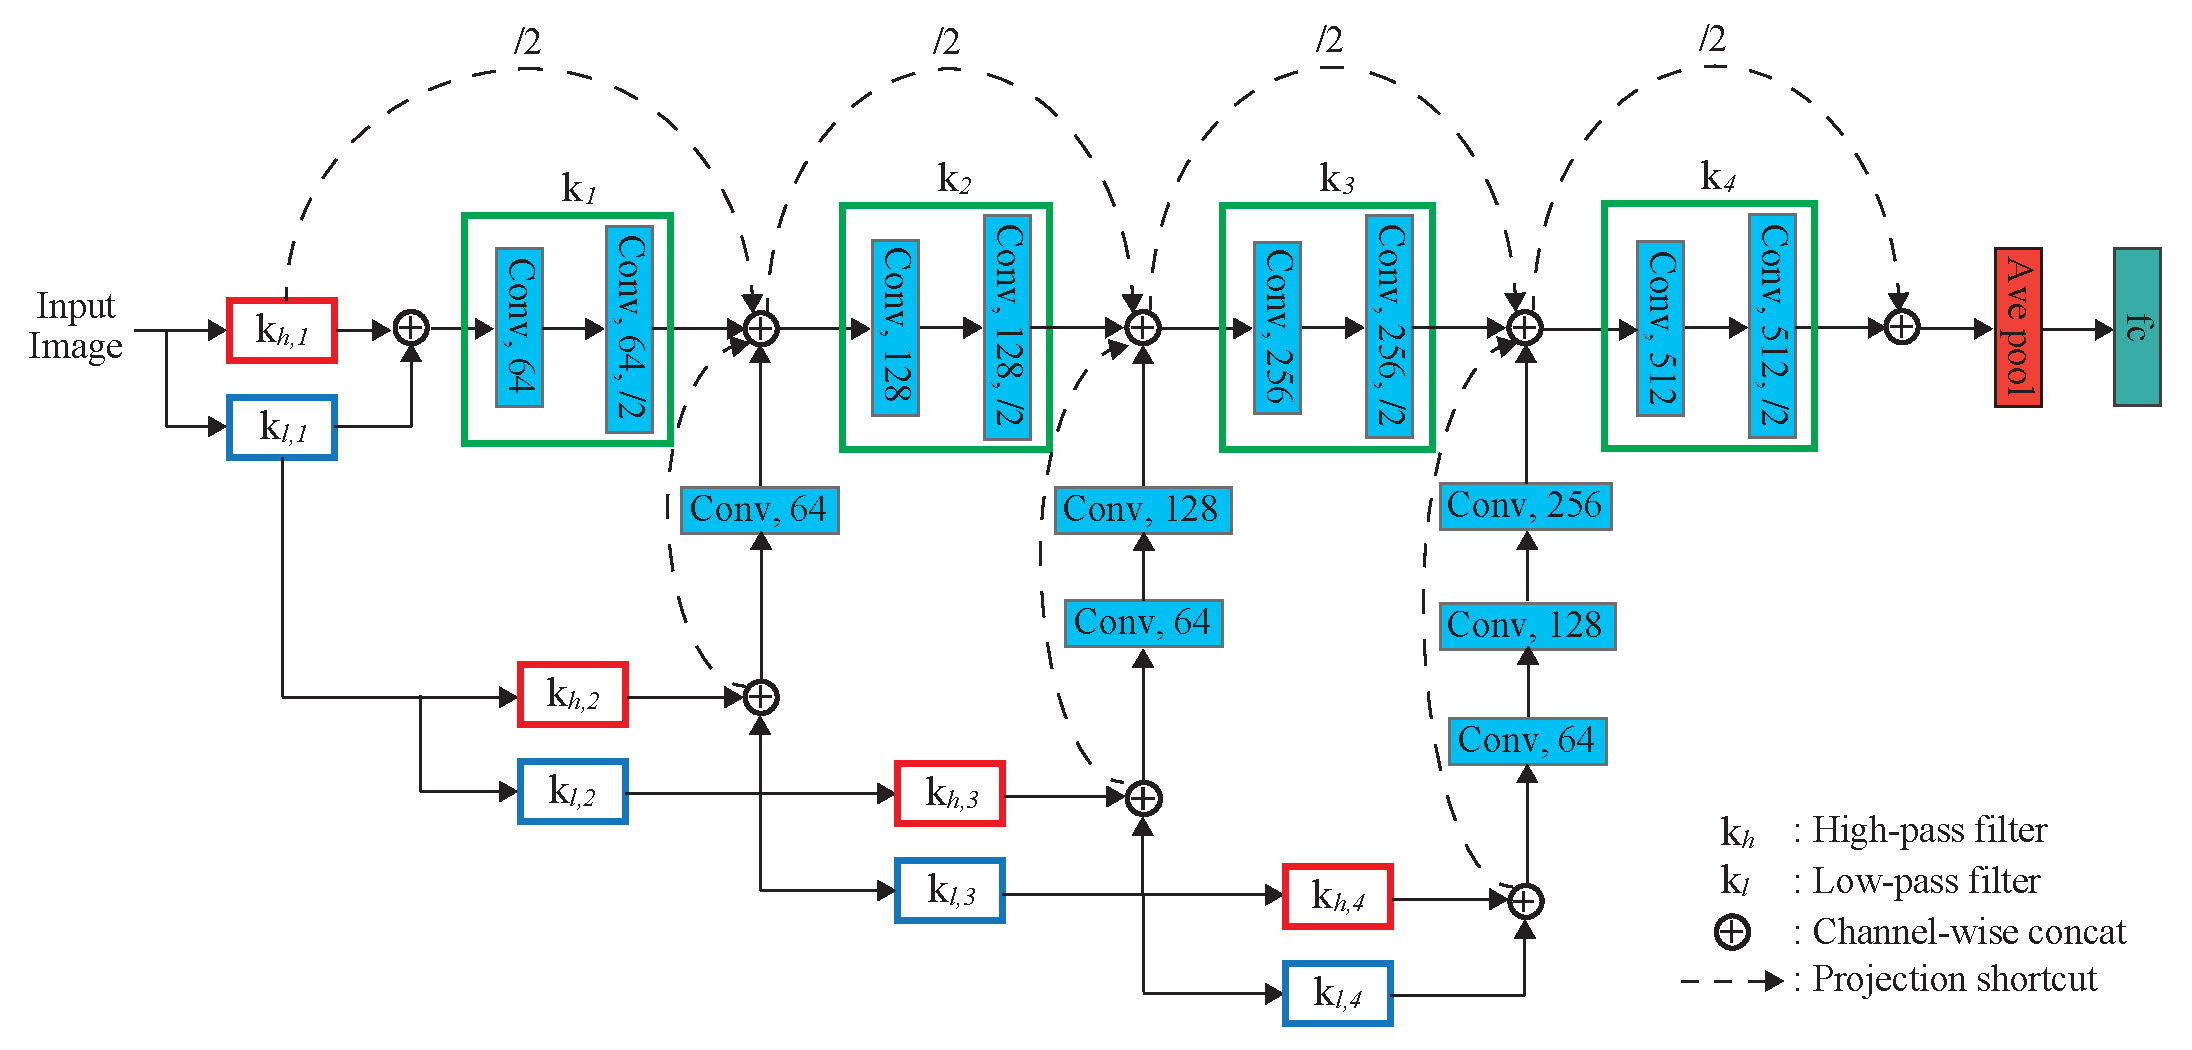
\includegraphics[width=\textwidth]{\imgpath/wavelet_CNN_3.pdf}
  \mycaption{Architecture using the DWT as a frontend to a CNN}{Figure 1 from
  \cite{fujieda_wavelet_2018}. Fujieda et.\ al.\ take a multiscale wavelet
  decomposition of the input before passing the input through a standard
  CNN\@. They learn convolutional layers independently on each subband and feed
  these back into the network at different depths, where the resolution of the
  subband and the network activations match.}
  \label{fig:ch6:fujieda}
\end{figure}

Several works also use wavelets in deep neural networks for super-resolution
\cite{guo_deep_2017} and for adding detail back into dense pixel-wise
segmentation tasks \cite{ma_detailed_2018}. These typically save wavelet
coefficients and use them for the reconstruction phase.

\section{Background and Notation}
We make use of the 2-D $Z$-transform to simplify our analysis:
%
\begin{equation}
  X(\zz) = \sum_{n_1}\sum_{n_2} x[n_1, n_2]z_1^{-n_1}z_2^{-n_2} =
  \sum_{\nn}x[c, \nn]\zz^{-\nn}
\end{equation}
%
As we are working with three dimensional arrays (two spatial and one channel) but are
only doing convolution in two, we introduce a slightly modified 2-D $Z$-transform
which includes the channel index:
%
\begin{equation}
  X(c, \zz) = \sum_{n_1}\sum_{n_2} x[c, n_1, n_2]z_1^{-n_1}z_2^{-n_2} =
  \sum_{\nn}x[c, \nn]\zz^{-\nn} \label{eq:ch6:ztransform}
\end{equation}
%
Recall that a typical convolutional
layer in a standard CNN gets the next layer's output in a two-step process:
%
\begin{align} 
  \cnndlact{y}{l+1}{f}{\nn} &= \sum_{c=0}^{C_l - 1} \cnndlact{x}{l}{c}{\nn} \conv \cnndfilt{l}{f}{c}{\nn}
    \label{eq:ch6:conv}\\
    \cnndlact{x}{l+1}{f}{\xy} & =  \sigma \left( \cnndlact{y}{l+1}{f}{\xy} \right) \label{eq:ch6:nonlin}
\end{align}
%
In shorthand, we can reduce the action of the convolutional layer in \eqref{eq:ch6:conv} to $H$, saying:
\begin{equation}
  y^{(l+1)} = Hx^{(l)}
\end{equation}
%
With the new $Z$-transform notation introduced in \eqref{eq:ch6:ztransform}, we
can rewrite \eqref{eq:ch6:conv} as:
%
\begin{equation}
  \cnnlact{Y}{l+1}{f}{\zz} = \sum_{c=0}^{C_l - 1} \cnnlact{X}{l}{c}{\zz} H_f^{(l)}(c, \zz)
\end{equation}
%
Note that we cannot rewrite \eqref{eq:ch6:nonlin} with $Z$-transforms as it is a nonlinear
operation.

Also recall that with multirate systems, upsampling by $M$ takes $X(z)$ to
$X(z^M)$ and downsampling by $M$ takes $X(z)$ to $\frac{1}{M}\sum_{k=0}^{M-1} X(W_M^k
z^{1/k})$ where $W_M^k = e^{\frac{j2\pi k}{M}}$. We will drop the $M$ subscript
below unless it is unclear of the sample rate change, simply using $W^k$.

\subsection{$\DTCWT$ Notation}
For this chapter, we will work with lots of $\DTCWT$ coefficients so we define
some slightly new notation here.

A $J$ scale $\DTCWT$ gives $6J+1$ coefficients, 6 sets of complex
bandpass coefficients for each scale (representing the oriented bands from 15 to 165
degrees) and 1 set of real lowpass coefficients. 
\begin{equation}
  \DTCWT_J(x) = \{ u_{lp}, u_{j,k} \}_{1\leq j\leq J, 1\leq k\leq 6}
  \label{eq:ch6:dtcwt_coeffs}
\end{equation}

Each of these coefficients then has size:
%
\begin{eqnarray}
  u_{lp} &\in & \reals[N\x C\x \frac{H}{2^{J-1}} \x \frac{W}{2^{J-1}}] \\
  u_{j,k} &\in & \complexes[N\x C\x \frac{H}{2^{J}}\x \frac{W}{2^{J}}]
\end{eqnarray}
%
Note that the lowpass coefficients are twice as large as in a fully decimated
transform, a feature of the redundancy of the $\DTCWT$.

If we ever want to refer to all the subbands at a given scale, we will
drop the $k$ subscript and call them $u_j$. Likewise, $u$ refers to the whole
set of $\DTCWT$ coefficients.

\section{Learning in Multiple Spaces}\label{sec:ch6:learning}

\begin{figure}[t]
  \centering
  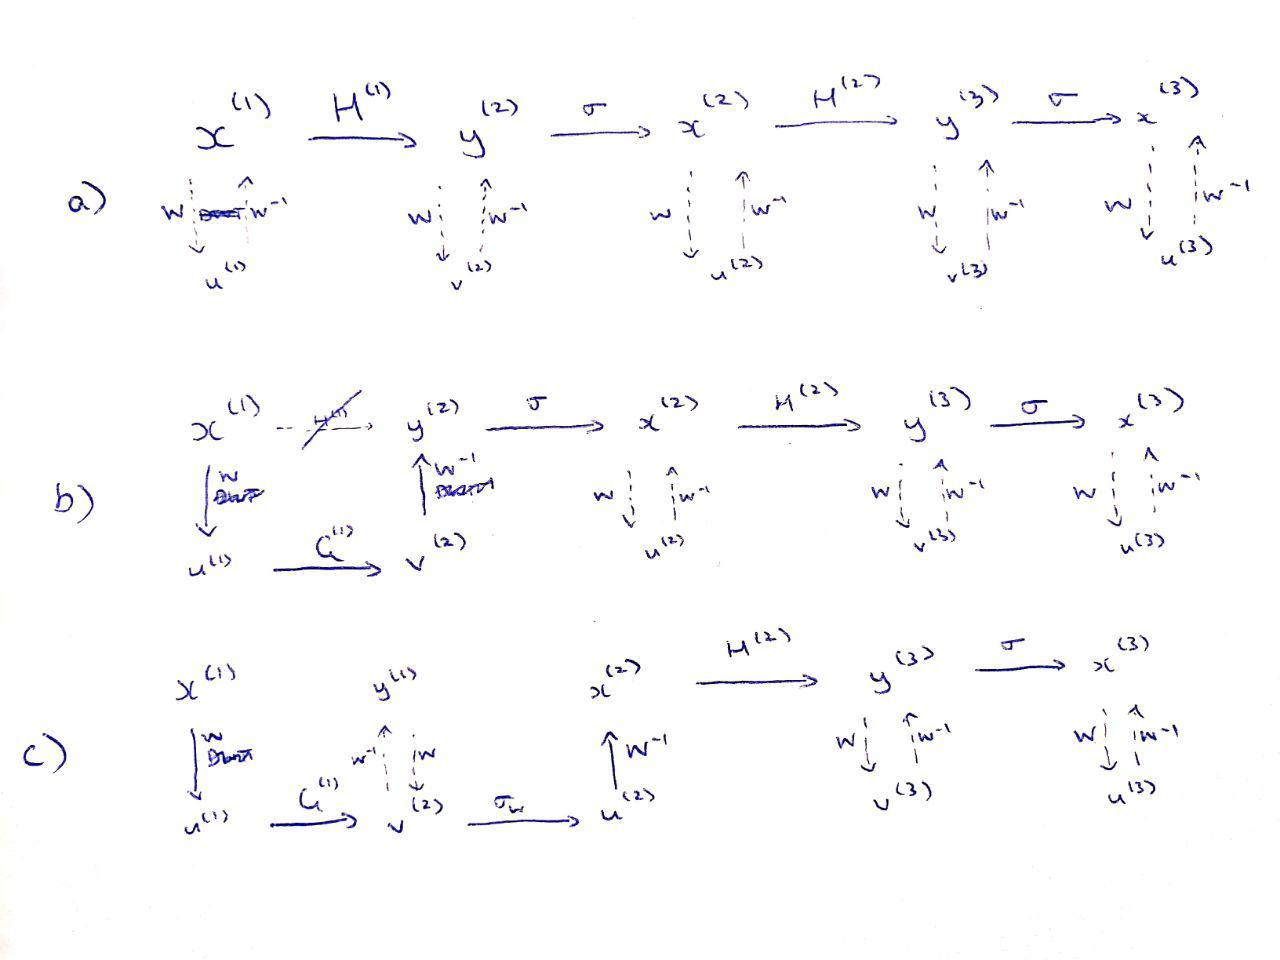
\includegraphics[width=0.8\textwidth]{\imgpath/fwd_chain.jpg}
  \mycaption{Proposed new forward pass in the wavelet domain}{Two network 
  layers with some possible options for processing. Solid lines denote the
  evaluation path and dashed lines indicate relationships. In (a) we see a
  regular convolutional neural network. We have included the dashed lines to
  make clear what we are denoting as $u$ and $v$ with respect to their
  equivalents $x$ and $y$. In (b) we get to $y^{(2)}$ through a different path.
  First we take the wavelet transform of $x^{(1)}$ to give $u^{(1)}$, apply a
  wavelet gain layer $G^{(1)}$, and take the inverse wavelet transform
  to give $y^{(2)}$. The cross through $H^{(1)}$ indicates that this
  path is no longer present. Note that there may not be any possible
  $G^{(1)}$ to make $y^{(2)}$ from (b) equal $y^{(2)}$ from (a). In
  (c) we have stayed in the wavelet domain longer, and applied a wavelet
  nonlinearity $\sigma_w$ to give $u^{(2)}$. We then return to the pixel domain
  to give $x^{(2)}$ and continue on from there in the pixel domain.}
  \label{fig:ch6:fwd_chain}
\end{figure}
At the beginning of each stage of a neural network we have the activations
$x^{(l)}$. Naturally, all of these activations have their equivalent wavelet
coefficients $u^{(l)}$. 

From \eqref{eq:ch6:conv}, convolutional layers also have intermediate
activations $y^{(l)}$. Let us differentiate these from the $x$ coefficients and
modify \eqref{eq:ch6:dtcwt_coeffs} to say the $\DTCWT$ of $y^{(l)}$ gives
$v^{(l)}$.

We now propose the \emph{wavelet gain layer} $G$.
The name `gain layer' comes from the inspiration for this chapter's work, in
that the first layer of CNN could theoretically be done in the wavelet domain by
setting subband gains to 0 and 1. 

The gain layer $G$ can be used instead of a convolutional layer. 
It is designed to work on the wavelet coefficients of an activation,
$u$ to give outputs $v$. 

This can be seen as breaking the convolutional path in
\autoref{fig:ch6:fwd_chain} and taking a new route to get to the next layer's
coefficients. From here, we can return to the pixel domain by taking the
corresponding inverse wavelet transform $W^{-1}$. Alternatively, we
can stay in the wavelet domain and apply wavelet based nonlinearities
for the lowpass $\sigma_{lp}$ and highpass $\sigma_{bp}$ coefficients
to give $u^{(l+1)}$. Ultimately we would like to explore
architecture design with arbitrary sections in the wavelet and pixel domain, but
to do this we must first explore: 
\begin{enumerate}[itemsep=0pt,parsep=5pt,topsep=0pt]
  \item How effective is $G$ at replacing $H$?
  \item What are effective wavelet nonlinearities $\sigma_{lp}$ and $\sigma_{bp}$?
\end{enumerate}

\subsection{The $\DTCWT$ Gain Layer}
To do the mixing across the $C_l$ channels at each subband, giving $C_{l+1}$
output channels, we introduce the learnable filters $g_{lp}, g_{j,k}$:
%
\begin{align}
  g_{lp} &\in \reals[C_{l+1}\x C_l\x k_{lp}\x k_{lp}] \label{eq:ch6:glp} \\
  g_{1,1} &\in \complexes[C_{l+1}\x C_l\x k_1\x k_1] \\
  g_{1,2} &\in \complexes[C_{l+1}\x C_l\x k_1\x k_1] \\
      & \vdots \nonumber \\
  g_{J,6} &\in \complexes[C_{l+1}\x C_l\x k_J\x k_J]  \label{eq:ch6:gj6}
\end{align}
%
where $k$ is the size of the mixing kernels. These could be $1\x 1$ for
simple gain control, or could be larger, say $3\x 3$, to do more complex
filtering on the subbands. Importantly, we can select the support size
differently for each subband.

With these gains we define the action of the gain layer $v = Gu$ to be:
\begin{align}
  v_{lp}[f, \nn] &=  \sum_{c=0}^{C_l-1} u_{lp}[c, \nn] \conv g_{lp}[f, c, \nn] \\
  v_{1,1}[f, \nn] &=  \sum_{c=0}^{C_l-1} u_{1,1}[c, \nn] \conv g_{1,1}[f, c, \nn] \\
  v_{1,2}[f, \nn] &=  \sum_{c=0}^{C_l-1} u_{1,2}[c, \nn] \conv g_{1,2}[f, c, \nn] \\
                  & \vdots \nonumber \\
  v_{J,6}[f, \nn] &=  \sum_{c=0}^{C_l-1} u_{J,6}[c, \nn] \conv g_{J,6}[f, c, \nn] 
\end{align}

Note that for complex signals $a, b$ the convolution $a \conv b$ is defined as $(a_r \conv
b_r - a_i \conv b_i) + j(a_r \conv b_i + a_i \conv b_r)$ (see \autoref{ch6:app:complex_weights}). 

The action of the gain layer with $J=1$ is is shown in
\autoref{fig:ch6:block_diagrams}.

\begin{figure}[t!]
  \centering
  % \resizebox{\textwidth}{!}{\begin{tikzpicture}[%
  path image/.style={%
    path picture={%
      \node at (path picture bounding box.center) {%
        \includegraphics[height=2.0cm]{#1}
      };
    }
  }, 
  path pic/.style={%
    path picture={%
      \node at (path picture bounding box.center) {%
        \includegraphics[height=0.8cm]{#1}
      };
    }
  }, 
  scale=0.6]
  \draw (-1, 0.8, 3.5) node {\Large{$x^{(l)}$}};
  \draw (8.5, 2.5, 0) node {\Large{$u^{(l)}$}};
  \draw (9.7, 2.3, 0) node {\Large{$\conv$}};
  \draw (11, 2.5, 0) node {\Large{$g^{(l)}$}};
  \draw (15, 2.5, 0) node {\Large{$v^{(l+1)}$}};
  \draw (18.5, 2.5, 0) node {\Large{$u^{(l+1)}$}};
  \draw (25, 0.8, 3.5) node {\Large{$x^{(l+1)}$}};
  \draw[<->] (10, -1, -2) -- (10, 0.9, -2) node[near end, right] {$C_{l+1}$};

  \draw (1.0, -2.5, -3) node {bandpass};
  \draw (2.0, -2.5, 14) node {lowpass};
  \draw [decorate,decoration={brace,mirror,amplitude=10pt,raise=4pt},yshift=0pt]
    (3.8,-2.5,-8) -- (4.8,-2.5,18) node [black,midway,xshift=0.8cm];
  \draw [->, fill=gray!30,ultra thick] (0.5, -2.5, 4) -- (2.5, -2.5, 4)
    node[midway, above] {$\DTCWT$};
  \tikzcuboid{
  shiftx=-2.5cm,
  shifty=-2.5cm,
  shiftz=7,
  scale=0.5,
  anglex=0, 
  angley=90, 
  anglez=230,
  dimx=3, 
  dimy=3, 
  dimz=6,
  densityx=1, 
  densityy=1, 
  densityz=1,
  shade=false,
  emphedge=true,
  shadeopacity=0,
  emphstyle/.style={rounded corners=0.2pt,line width=0.3mm},
  front/.style={draw=blue!50!white,fill=blue!50!white},%
  right/.style={draw=blue!50!white,fill=blue!50!white},%
  top/.style={draw=blue!50!white,fill=blue!50!white},%
  drawxdims=true,
  dimxval=W,
  drawydims=true,
  dimyval=H,
  drawzdims=true,
  dimzval=C_l,
  }

  % Draw the 6 subband activations and their filters
  \foreach \i in {1,...,5} {
    \tikzcuboid{
    shiftx=6cm,
    shifty=-2.0cm,
    shiftz=-15+5*\i,
    scale=0.5,
    dimx=2, dimy=2, dimz=3,
    densityx=4, densityy=4, densityz=2,
    drawxdims=false,
    drawydims=false,
    dimzval=C_l,
    drawzdims=false,
    front/.style={draw=blue!90!white,fill=blue!90!white},%
    right/.style={draw=blue!90!white,fill=blue!90!white},%
    top/.style={draw=blue!90!white,fill=blue!90!white},%
    }
    \tikzcuboid{
    dimz=2,
    shiftx=12.0cm,
    }
    \tikzcuboid{
    shiftx=16.0cm,
    }
    \draw [->, fill=gray!30,ultra thick] (9.8+0.08*\i, -1.5, -7+2.5*\i) -- (10.8+0.08*\i, -1.5, -7+2.5*\i);
      % node[midway, above] {$\sigma_w$};
    \draw [->, fill=gray!30,ultra thick] (13.8+0.08*\i, -1.5, -7+2.5*\i) -- (14.8+0.08*\i, -1.5, -7+2.5*\i)
      node[midway, above] {$\sigma_w$};

    \tikzcuboid{
    shiftx=8.5cm,
    shifty=-1.0cm,
    shiftz=-15+5*\i,
    dimx=0.4, dimy=0.4, dimz=3,
    densityx=5, densityy=5, densityz=2,
    front/.style={draw=red!90!white,fill=red!90!white},%
    right/.style={draw=red!90!white,fill=red!90!white},%
    top/.style={draw=red!90!white,fill=red!90!white},%
    }
    \tikzcuboid{
    shifty=-1.5cm,
    }
    \tikzcuboid{
    shifty=-2.0cm,
    }
    \tikzcuboid{
    shifty=-2.5cm,
    }
    % \draw (8cm, -1.8cm, -15+5*\i) node {$\vdots$};
  }
  \tikzcuboid{
  shiftx=6cm,
  shifty=-2.0cm,
  shiftz=15,
  scale=0.5,
  dimx=2, dimy=2, dimz=3,
  densityx=4, densityy=4, densityz=2,
  dimxval=\frac{W}{2},
  drawxdims=true,
  dimyval=\frac{H}{2},
  drawydims=true,
  dimzval=C_l,
  drawzdims=true,
  front/.style={draw=blue!90!white,fill=blue!90!white},%
  right/.style={draw=blue!90!white,fill=blue!90!white},%
  top/.style={draw=blue!90!white,fill=blue!90!white},%
  }
  \tikzcuboid{
  shiftx=12.0cm,
  dimz=2,
  dimzval=C_{l+1},
  }
  \tikzcuboid{
  shiftx=16.0cm,
  drawxdims=false,
  drawydims=false,
  drawzdims=false
  }
  \draw [->, fill=gray!30,ultra thick] (9.8+6*0.08, -1.5, 8) -- (10.8+6*0.08, -1.5, 8);
    % node[midway, above] {$\sigma_w$};
  \draw [->, fill=gray!30,ultra thick] (13.8+6*0.08, -1.5, 8) -- (14.8+6*0.08, -1.5, 8)
      node[midway, above] {$\sigma_w$};
  \tikzcuboid{
  shiftx=8.5cm,
  shifty=-1.0cm,
  shiftz=15,
  dimx=0.4, dimy=0.4, dimz=3,
  drawxdims=false,
  drawydims=false,
  drawzdims=false,
  densityx=5, densityy=5, densityz=2,
  front/.style={draw=red!90!white,fill=red!90!white},%
  right/.style={draw=red!90!white,fill=red!90!white},%
  top/.style={draw=red!90!white,fill=red!90!white},%
  }
  \tikzcuboid{
  shifty=-1.5cm,
  }
  \tikzcuboid{
  shifty=-2.0cm,
  }
  \tikzcuboid{
  shifty=-2.5cm,
  }

  % Draw the lowpass activation and its set of filters
  \tikzcuboid{
  shiftx=6cm,
  shifty=-2.0cm,
  shiftz=35,
  scale=0.5,
  dimx=3, dimy=3, dimz=4,
  densityx=4, densityy=4, densityz=2,
  dimxval=W,
  drawxdims=true,
  dimyval=H,
  drawydims=true,
  dimzval=C_l,
  drawzdims=true,
  front/.style={draw=blue!50!white,fill=blue!50!white},%
  right/.style={draw=blue!50!white,fill=blue!50!white},%
  top/.style={draw=blue!50!white,fill=blue!50!white},%
  }
  \tikzcuboid{
  shiftx=12.0cm,
  dimz=2,
  drawxdims=true,
  drawydims=true,
  dimzval=C_{l+1},
  drawzdims=true
  }
  \tikzcuboid{
  shiftx=16.0cm,
  drawxdims=false,
  drawydims=false,
  drawzdims=false,
  }
  \draw [->, fill=gray!30,ultra thick] (11.2, -1.5, 17.5) -- (12.0, -1.5, 17.5);
    % node[midway, above] {$\sigma_w$};
  \draw [->, fill=gray!30,ultra thick] (15.5, -1.5, 17.5) -- (16.5, -1.5, 17.5)
    node[midway, above] {$\sigma_w$};

  \tikzcuboid{
  shiftx=9cm,
  shifty=-2.75cm,
  dimx=0.8, dimy=0.8, dimz=3,
  drawxdims=false,
  drawydims=false,
  drawzdims=false,
  densityx=5, densityy=5, densityz=2,
  front/.style={draw=red!50!white,fill=red!50!white},%
  right/.style={draw=red!50!white,fill=red!50!white},%
  top/.style={draw=red!50!white,fill=red!50!white},%
  }
  \tikzcuboid{
  shifty=-2.00cm,
  }
  \tikzcuboid{
  shifty=-1.25cm,
  }
  \tikzcuboid{
  shifty=-0.5cm,
  }
  \tikzcuboid{
  shiftx=23cm,
  shifty=-2.5cm,
  shiftz=7,
  scale=0.5,
  anglex=0, 
  angley=90, 
  anglez=230,
  dimx=3, 
  dimy=3, 
  dimz=6,
  densityx=1, 
  densityy=1, 
  densityz=1,
  shade=false,
  emphedge=true,
  shadeopacity=0,
  emphstyle/.style={rounded corners=0.2pt,line width=0.3mm},
  front/.style={draw=blue!50!white,fill=blue!50!white},%
  right/.style={draw=blue!50!white,fill=blue!50!white},%
  top/.style={draw=blue!50!white,fill=blue!50!white},%
  drawxdims=true,
  dimxval=W,
  drawydims=true,
  dimyval=H,
  drawzdims=true,
  dimzval=C_{l+1},
  }
  % \draw (0, .3, 0) node {\large{$x^{(l)}$}};
  \draw [decorate,decoration={brace,amplitude=10pt,raise=4pt},yshift=0pt]
    (16.5,-2.5,-8) -- (18,-2.5,18) node [black,midway,xshift=0.8cm];
  \draw [->, fill=gray!30,ultra thick] (19, -2.5, 4) -- (21.5, -2.5, 4)
    node[midway, above] {$\DTCWT^{-1}$};

\end{tikzpicture}
}
  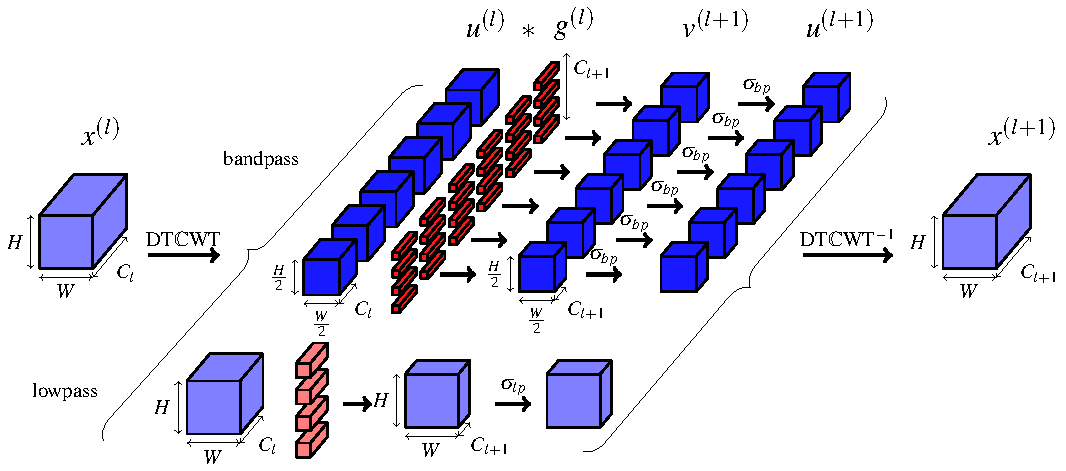
\includegraphics[width=\textwidth]{\imgpath/block_diagram_dtcwt}
  \label{fig:ch6:dtcwt_blk_diagram}
  \mycaption{Diagram of proposed method to learn in the wavelet domain}{
  Activations are shaded blue and learned parameters red. Deeper shades of blue
  and red indicate complex valued activations/weights, and lighter values
  indicate real valued activations/weights. The input $x^{(l)}\in
  \mathbb{R}^{C_l\x H\x W}$ is taken into the wavelet domain (here $J=1$) and each 
  subband is mixed independently with $C_{l+1}$ sets of convolutional filters.
  After mixing, a possible wavelet nonlinearity $\sigma_w$ is applied to the
  subbands, before returning to the pixel domain with an inverse wavelet
  transform.}
  \label{fig:ch6:block_diagrams}
\end{figure}

\subsubsection{The Output}
% \begin{figure}[t]
  % \centering
  % \begin{tikzpicture}
    \matrix (m1) [row sep=5mm, column sep=6mm,align=center,anchor=center]
	{
	%--------------------------------------------------------------------
		\node[coordinate]                  (m00) {};    &
		\node[coordinate]                  (m01) {};          &
		\node[dspsquare]                   (m02) {$A_r(z)$};          &
		\node[circle,draw,inner sep=1pt]   (m03) {\downsamplertext{M}}; &
		\node[dspnodeopen,dsp/label=above] (m04) {$U_r(z)$};          &
    \node[rectangle,draw,inner sep=2pt](m05) {$G_{r}(z)$}; &
		\node[dspnodeopen,dsp/label=above] (m06) {$V_r(z)$};          &
		\node[circle,draw,inner sep=1pt]   (m07) {\upsamplertext{M}}; &
		\node[dspsquare]                   (m08) {$S_r(z)$};          &
		\node[coordinate]                  (m09) {};          &
		\node[coordinate]                  (m0X) {};          \\
		%--------------------------------------------------------------------
		\node[]                            (m10) {$X(z)$};          &
		\node[coordinate]                  (m11) {};          &
		\node[coordinate]                  (m12) {};    &
		\node[coordinate]                  (m13) {};          &
		\node[coordinate]                  (m14) {};    &
		\node[coordinate]                  (m15) {};          &
		\node[coordinate]                  (m16) {};    &
		\node[coordinate]                  (m17) {};          &
		\node[coordinate]                  (m18) {};    &
		\node[dspadder]                    (m19) {};          &
    \node[]                            (m1X) {$Y(z)$};          \\
		%--------------------------------------------------------------------
		\node[coordinate]                  (m20) {};    &
		\node[coordinate]                  (m21) {};          &
		\node[dspsquare]                   (m22) {$A_i(z)$};          &
		\node[circle,draw,inner sep=1pt]   (m23) {\downsamplertext{M}}; &
		\node[dspnodeopen,dsp/label=below] (m24) {$U_i(z)$};          &
      \node[rectangle,draw,inner sep=2pt](m25) {$G_{r}(z)$}; &
		\node[dspnodeopen,dsp/label=below] (m26) {$V_i(z)$};          &
		\node[circle,draw,inner sep=1pt]   (m27) {\upsamplertext{M}}; &
		\node[dspsquare]                   (m28) {$S_i(z)$};          &
		\node[coordinate]                  (m29) {};          &
		\node[coordinate]                  (m2X) {};          \\
		%--------------------------------------------------------------------
  };
	\draw[dspline] (m10) -- (m11);
	\draw[dspline] (m11) -- (m01);
	\draw[dspline] (m11) -- (m21);
	\foreach \i in {0,2} {
    	\draw[dspconn] (m\i1) -- (m\i2);
    	\draw[dspconn] (m\i2) -- (m\i3);
    	\draw[dspline] (m\i3) -- (m\i4);
    	\draw[dspconn] (m\i4) -- (m\i5);
    	\draw[dspline] (m\i5) -- (m\i6);
    	\draw[dspconn] (m\i6) -- (m\i7);
    	\draw[dspconn] (m\i7) -- (m\i8);
    	\draw[dspline] (m\i8) -- (m\i9);
	}
	%\draw[dspflow] (m04) --  (m06);
	%\draw[dspflow] (m24) -- (m26);
  \draw[dspconn] (m24) -- node[draw,pos=0.7,inner sep=2pt,fill=white] {$-G_{i}(z)$} (m06);
  \draw[dspconn] (m04) -- node[draw,pos=0.7,inner sep=2pt,fill=white] {$G_{i}(z)$} (m26);
  \draw[dspconn] (m09) -- (m19);
  \draw[dspconn] (m29) -- (m19);
	\draw[dspconn] (m19) -- (m1X);
	
\end{tikzpicture}


  % \mycaption{Block Diagram of a single channel 1-D $\DTCWT$ Gain Layer}{Here we show the real and
  % imaginary trees for a single subband. Note that while it may look similar to 
  % a DWT block diagram, this diagram represents the two trees for one subband rather
  % than a single tree with a pair of subbands. The gain layer does a complex
  % multiply, using both the real and imaginary parts of the decomposed signal.
  % This preserves the shift invariance of the $\DTCWT$ for the reconstructed
  % signal $Y$.
  % }
  % \label{fig:ch6:dtcwt_gain}
% \end{figure}
\begin{figure}[t]
  \centering
  \makebox[\linewidth][c]{
  \subfloat[]{%
    % \includegraphics[width=\textwidth]{\imgpath/dtcwt_gain}
    \begin{tikzpicture}
    \matrix (m1) [row sep=5mm, column sep=6mm,align=center,anchor=center]
	{
	%--------------------------------------------------------------------
		\node[coordinate]                  (m00) {};    &
		\node[coordinate]                  (m01) {};          &
		\node[dspsquare]                   (m02) {$A_r(z)$};          &
		\node[circle,draw,inner sep=1pt]   (m03) {\downsamplertext{M}}; &
		\node[dspnodeopen,dsp/label=above] (m04) {$U_r(z)$};          &
    \node[rectangle,draw,inner sep=2pt](m05) {$G_{r}(z)$}; &
		\node[dspnodeopen,dsp/label=above] (m06) {$V_r(z)$};          &
		\node[circle,draw,inner sep=1pt]   (m07) {\upsamplertext{M}}; &
		\node[dspsquare]                   (m08) {$S_r(z)$};          &
		\node[coordinate]                  (m09) {};          &
		\node[coordinate]                  (m0X) {};          \\
		%--------------------------------------------------------------------
		\node[]                            (m10) {$X(z)$};          &
		\node[coordinate]                  (m11) {};          &
		\node[coordinate]                  (m12) {};    &
		\node[coordinate]                  (m13) {};          &
		\node[coordinate]                  (m14) {};    &
		\node[coordinate]                  (m15) {};          &
		\node[coordinate]                  (m16) {};    &
		\node[coordinate]                  (m17) {};          &
		\node[coordinate]                  (m18) {};    &
		\node[dspadder]                    (m19) {};          &
    \node[]                            (m1X) {$Y(z)$};          \\
		%--------------------------------------------------------------------
		\node[coordinate]                  (m20) {};    &
		\node[coordinate]                  (m21) {};          &
		\node[dspsquare]                   (m22) {$A_i(z)$};          &
		\node[circle,draw,inner sep=1pt]   (m23) {\downsamplertext{M}}; &
		\node[dspnodeopen,dsp/label=below] (m24) {$U_i(z)$};          &
      \node[rectangle,draw,inner sep=2pt](m25) {$G_{r}(z)$}; &
		\node[dspnodeopen,dsp/label=below] (m26) {$V_i(z)$};          &
		\node[circle,draw,inner sep=1pt]   (m27) {\upsamplertext{M}}; &
		\node[dspsquare]                   (m28) {$S_i(z)$};          &
		\node[coordinate]                  (m29) {};          &
		\node[coordinate]                  (m2X) {};          \\
		%--------------------------------------------------------------------
  };
	\draw[dspline] (m10) -- (m11);
	\draw[dspline] (m11) -- (m01);
	\draw[dspline] (m11) -- (m21);
	\foreach \i in {0,2} {
    	\draw[dspconn] (m\i1) -- (m\i2);
    	\draw[dspconn] (m\i2) -- (m\i3);
    	\draw[dspline] (m\i3) -- (m\i4);
    	\draw[dspconn] (m\i4) -- (m\i5);
    	\draw[dspline] (m\i5) -- (m\i6);
    	\draw[dspconn] (m\i6) -- (m\i7);
    	\draw[dspconn] (m\i7) -- (m\i8);
    	\draw[dspline] (m\i8) -- (m\i9);
	}
	%\draw[dspflow] (m04) --  (m06);
	%\draw[dspflow] (m24) -- (m26);
  \draw[dspconn] (m24) -- node[draw,pos=0.7,inner sep=2pt,fill=white] {$-G_{i}(z)$} (m06);
  \draw[dspconn] (m04) -- node[draw,pos=0.7,inner sep=2pt,fill=white] {$G_{i}(z)$} (m26);
  \draw[dspconn] (m09) -- (m19);
  \draw[dspconn] (m29) -- (m19);
	\draw[dspconn] (m19) -- (m1X);
	
\end{tikzpicture}


    \label{fig:ch6:fwd_pass}
    }}
   \newline
  \makebox[\linewidth][c]{
  \subfloat[]{%
    \begin{tikzpicture}
    \matrix (m1) [row sep=5mm, column sep=6mm,align=center,anchor=center]
	{
	% %--------------------------------------------------------------------
		% \node[coordinate]                  (m00) {};    &
		% \node[coordinate]                  (m01) {};          &
		% \node[dspsquare]                   (m02) {$A(z)$};          &
		% \node[circle,draw,inner sep=1pt]   (m03) {\downsamplertext{M}}; &
		% \node[dspnodeopen,dsp/label=above] (m04) {$V_r(z)$};          &
		% \node[rectangle,draw,inner sep=2pt](m05) {$G_r(z)$}; &
		% \node[dspnodeopen,dsp/label=above] (m06) {$W_r(z)$};          &
		% \node[circle,draw,inner sep=1pt]   (m07) {\upsamplertext{M}}; &
		% \node[dspsquare]                   (m08) {$C(z)$};          &
		% \node[coordinate]                  (m09) {};          &
		% \node[coordinate]                  (m0X) {};          \\
		% %--------------------------------------------------------------------
		% \node[]                            (m10) {$X(z)$};          &
		% \node[coordinate]                  (m11) {};          &
		% \node[coordinate]                  (m12) {};    &
		% \node[coordinate]                  (m13) {};          &
		% \node[coordinate]                  (m14) {};    &
		% \node[coordinate]                  (m15) {};          &
		% \node[coordinate]                  (m16) {};    &
		% \node[coordinate]                  (m17) {};          &
		% \node[coordinate]                  (m18) {};    &
		% \node[dspadder]                    (m19) {};          &
    % \node[]                            (m1X) {$Y(z)$};          \\
		% %--------------------------------------------------------------------
		% \node[coordinate]                  (m20) {};    &
		% \node[coordinate]                  (m21) {};          &
		% \node[dspsquare]                   (m22) {$B(z)$};          &
		% \node[circle,draw,inner sep=1pt]   (m23) {\downsamplertext{M}}; &
		% \node[dspnodeopen,dsp/label=below] (m24) {$V_i(z)$};          &
		% \node[rectangle,draw,inner sep=2pt](m25) {$G_r(z)$}; &
		% \node[dspnodeopen,dsp/label=below] (m26) {$W_i(z)$};          &
		% \node[circle,draw,inner sep=1pt]   (m27) {\upsamplertext{M}}; &
		% \node[dspsquare]                   (m28) {$D(z)$};          &
		% \node[coordinate]                  (m29) {};          &
		% \node[coordinate]                  (m2X) {};          \\
		% %--------------------------------------------------------------------
		% &&&&&&&&& \\
		\node[coordinate]                  (m00a) {};    &
		\node[coordinate]                  (m01a) {};          &
		\node[dspsquare]                   (m02a) {$A\left(z^{-1}\right)$};          &
		\node[circle,draw,inner sep=1pt]   (m03a) {\upsamplertext{M}}; &
		\node[dspnodeopen,dsp/label=above] (m04a) {$\Delta U_r(z)$};          &
		%\node[coordinate]                  (m05) {}; &
		\node[rectangle,draw,inner sep=2pt](m05a) {$G_r\left(z^{-1}\right)$}; &
		\node[dspnodeopen,dsp/label=above] (m06a) {$\Delta V_r(z)$};          &
		\node[circle,draw,inner sep=1pt]   (m07a) {\downsamplertext{M}}; &
		\node[dspsquare]                   (m08a) {$C\left(z^{-1}\right)$};          &
		\node[coordinate]                  (m09a) {};          &
		\node[coordinate]                  (m0Xa) {};          \\
		%--------------------------------------------------------------------
		%\node[coordinate]  (m10) {$\Delta X(z)$};          &
    \node[]                            (m10a) {$\Delta X(z)$}; &
		\node[dspadder]                    (m11a) {};          &
		\node[coordinate]                  (m12a) {};    &
		\node[coordinate]                  (m13a) {};          &
		\node[coordinate]                  (m14a) {};    &
		\node[coordinate]                  (m15a) {};          &
		\node[coordinate]                  (m16a) {};    &
		\node[coordinate]                  (m17a) {};          &
		\node[coordinate]                  (m18a) {};    &
		\node[coordinate]                  (m19a) {};          &
		\node[]                            (m1Xa) {$\Delta Y(z)$};          \\
		%--------------------------------------------------------------------
		\node[coordinate]                  (m20a) {};    &
		\node[coordinate]                  (m21a) {};          &
		\node[dspsquare]                   (m22a) {$B\left(z^{-1}\right)$};          &
		\node[circle,draw,inner sep=1pt]   (m23a) {\upsamplertext{M}}; &
		\node[dspnodeopen,dsp/label=below] (m24a) {$\Delta U_i(z)$};          &
		%\node[coordinate]                  (m25) {}; &
		\node[rectangle,draw,inner sep=2pt](m25a) {$G_r\left(z^{-1}\right)$}; &
		\node[dspnodeopen,dsp/label=below] (m26a) {$\Delta V_i(z)$};          &
		\node[circle,draw,inner sep=1pt]   (m27a) {\downsamplertext{M}}; &
		\node[dspsquare]                   (m28a) {$D\left(z^{-1}\right)$};          &
		\node[coordinate]                  (m29a) {};          &
		\node[coordinate]                  (m2Xa) {};          \\
		%--------------------------------------------------------------------
	};
	% \draw[dspline] (m10) -- (m11);
	% \draw[dspline] (m11) -- (m01);
	% \draw[dspline] (m11) -- (m21);
	% \foreach \i in {0,2} {
      % \draw[dspconn] (m\i1) -- (m\i2);
      % \draw[dspconn] (m\i2) -- (m\i3);
      % \draw[dspline] (m\i3) -- (m\i4);
      % \draw[dspconn] (m\i4) -- (m\i5);
      % \draw[dspline] (m\i5) -- (m\i6);
      % \draw[dspconn] (m\i6) -- (m\i7);
      % \draw[dspconn] (m\i7) -- (m\i8);
      % \draw[dspline] (m\i8) -- (m\i9);
	% }
	% %\draw[dspflow] (m04) --  (m06);
	% %\draw[dspflow] (m24) -- (m26);
	% \draw[dspconn] (m24) -- node[draw,pos=0.7,inner sep=2pt,fill=white] {$-G_i(z)$} (m06);
	% \draw[dspconn] (m04) -- node[draw,pos=0.7,inner sep=2pt,fill=white] {$G_i(z)$} (m26);
	% \draw[dspconn] (m09) -- (m19);
	% \draw[dspconn] (m29) -- (m19);
	% \draw[dspconn] (m19) -- (m1X);
	\draw[dspconn] (m11a) -- (m10a);
	\draw[dspconn] (m01a) -- (m11a);
	\draw[dspconn] (m21a) -- (m11a);
	\foreach \i in {0,2} {
    	\draw[dspconn] (m\i9a) -- (m\i8a);
    	\draw[dspconn] (m\i8a) -- (m\i7a);
    	\draw[dspline] (m\i7a) -- (m\i6a);
    	\draw[dspconn] (m\i6a) -- (m\i5a);
    	\draw[dspline] (m\i5a) -- (m\i4a);
    	\draw[dspconn] (m\i4a) -- (m\i3a);
    	\draw[dspconn] (m\i3a) -- (m\i2a);
    	\draw[dspline] (m\i2a) -- (m\i1a);
	}
	%\draw[dspflow] (m04) --  (m06);
	%\draw[dspflow] (m24) -- (m26);
	\draw[dspconn] (m06a) -- node[draw,pos=0.7,inner sep=2pt,fill=white] {$-G_i\left(z^{-1}\right)$} (m24a);
	\draw[dspconn] (m26a) -- node[draw,pos=0.7,inner sep=2pt,fill=white] {$G_i\left(z^{-1}\right)$} (m04a);
	\draw[dspline] (m09a) -- (m19a);
	\draw[dspline] (m29a) -- (m19a);
	\draw[dspline] (m19a) -- (m1Xa);
	
\end{tikzpicture}

    % \includegraphics[width=\textwidth]{\imgpath/gain_layer}
    \label{fig:ch6:bwd_pass}
  }}
  % \begin{tikzpicture}
    \matrix (m1) [row sep=5mm, column sep=6mm,align=center,anchor=center]
	{
	% %--------------------------------------------------------------------
		% \node[coordinate]                  (m00) {};    &
		% \node[coordinate]                  (m01) {};          &
		% \node[dspsquare]                   (m02) {$A(z)$};          &
		% \node[circle,draw,inner sep=1pt]   (m03) {\downsamplertext{M}}; &
		% \node[dspnodeopen,dsp/label=above] (m04) {$V_r(z)$};          &
		% \node[rectangle,draw,inner sep=2pt](m05) {$G_r(z)$}; &
		% \node[dspnodeopen,dsp/label=above] (m06) {$W_r(z)$};          &
		% \node[circle,draw,inner sep=1pt]   (m07) {\upsamplertext{M}}; &
		% \node[dspsquare]                   (m08) {$C(z)$};          &
		% \node[coordinate]                  (m09) {};          &
		% \node[coordinate]                  (m0X) {};          \\
		% %--------------------------------------------------------------------
		% \node[]                            (m10) {$X(z)$};          &
		% \node[coordinate]                  (m11) {};          &
		% \node[coordinate]                  (m12) {};    &
		% \node[coordinate]                  (m13) {};          &
		% \node[coordinate]                  (m14) {};    &
		% \node[coordinate]                  (m15) {};          &
		% \node[coordinate]                  (m16) {};    &
		% \node[coordinate]                  (m17) {};          &
		% \node[coordinate]                  (m18) {};    &
		% \node[dspadder]                    (m19) {};          &
    % \node[]                            (m1X) {$Y(z)$};          \\
		% %--------------------------------------------------------------------
		% \node[coordinate]                  (m20) {};    &
		% \node[coordinate]                  (m21) {};          &
		% \node[dspsquare]                   (m22) {$B(z)$};          &
		% \node[circle,draw,inner sep=1pt]   (m23) {\downsamplertext{M}}; &
		% \node[dspnodeopen,dsp/label=below] (m24) {$V_i(z)$};          &
		% \node[rectangle,draw,inner sep=2pt](m25) {$G_r(z)$}; &
		% \node[dspnodeopen,dsp/label=below] (m26) {$W_i(z)$};          &
		% \node[circle,draw,inner sep=1pt]   (m27) {\upsamplertext{M}}; &
		% \node[dspsquare]                   (m28) {$D(z)$};          &
		% \node[coordinate]                  (m29) {};          &
		% \node[coordinate]                  (m2X) {};          \\
		% %--------------------------------------------------------------------
		% &&&&&&&&& \\
		\node[coordinate]                  (m00a) {};    &
		\node[coordinate]                  (m01a) {};          &
		\node[dspsquare]                   (m02a) {$A\left(z^{-1}\right)$};          &
		\node[circle,draw,inner sep=1pt]   (m03a) {\upsamplertext{M}}; &
		\node[dspnodeopen,dsp/label=above] (m04a) {$\Delta U_r(z)$};          &
		%\node[coordinate]                  (m05) {}; &
		\node[rectangle,draw,inner sep=2pt](m05a) {$G_r\left(z^{-1}\right)$}; &
		\node[dspnodeopen,dsp/label=above] (m06a) {$\Delta V_r(z)$};          &
		\node[circle,draw,inner sep=1pt]   (m07a) {\downsamplertext{M}}; &
		\node[dspsquare]                   (m08a) {$C\left(z^{-1}\right)$};          &
		\node[coordinate]                  (m09a) {};          &
		\node[coordinate]                  (m0Xa) {};          \\
		%--------------------------------------------------------------------
		%\node[coordinate]  (m10) {$\Delta X(z)$};          &
    \node[]                            (m10a) {$\Delta X(z)$}; &
		\node[dspadder]                    (m11a) {};          &
		\node[coordinate]                  (m12a) {};    &
		\node[coordinate]                  (m13a) {};          &
		\node[coordinate]                  (m14a) {};    &
		\node[coordinate]                  (m15a) {};          &
		\node[coordinate]                  (m16a) {};    &
		\node[coordinate]                  (m17a) {};          &
		\node[coordinate]                  (m18a) {};    &
		\node[coordinate]                  (m19a) {};          &
		\node[]                            (m1Xa) {$\Delta Y(z)$};          \\
		%--------------------------------------------------------------------
		\node[coordinate]                  (m20a) {};    &
		\node[coordinate]                  (m21a) {};          &
		\node[dspsquare]                   (m22a) {$B\left(z^{-1}\right)$};          &
		\node[circle,draw,inner sep=1pt]   (m23a) {\upsamplertext{M}}; &
		\node[dspnodeopen,dsp/label=below] (m24a) {$\Delta U_i(z)$};          &
		%\node[coordinate]                  (m25) {}; &
		\node[rectangle,draw,inner sep=2pt](m25a) {$G_r\left(z^{-1}\right)$}; &
		\node[dspnodeopen,dsp/label=below] (m26a) {$\Delta V_i(z)$};          &
		\node[circle,draw,inner sep=1pt]   (m27a) {\downsamplertext{M}}; &
		\node[dspsquare]                   (m28a) {$D\left(z^{-1}\right)$};          &
		\node[coordinate]                  (m29a) {};          &
		\node[coordinate]                  (m2Xa) {};          \\
		%--------------------------------------------------------------------
	};
	% \draw[dspline] (m10) -- (m11);
	% \draw[dspline] (m11) -- (m01);
	% \draw[dspline] (m11) -- (m21);
	% \foreach \i in {0,2} {
      % \draw[dspconn] (m\i1) -- (m\i2);
      % \draw[dspconn] (m\i2) -- (m\i3);
      % \draw[dspline] (m\i3) -- (m\i4);
      % \draw[dspconn] (m\i4) -- (m\i5);
      % \draw[dspline] (m\i5) -- (m\i6);
      % \draw[dspconn] (m\i6) -- (m\i7);
      % \draw[dspconn] (m\i7) -- (m\i8);
      % \draw[dspline] (m\i8) -- (m\i9);
	% }
	% %\draw[dspflow] (m04) --  (m06);
	% %\draw[dspflow] (m24) -- (m26);
	% \draw[dspconn] (m24) -- node[draw,pos=0.7,inner sep=2pt,fill=white] {$-G_i(z)$} (m06);
	% \draw[dspconn] (m04) -- node[draw,pos=0.7,inner sep=2pt,fill=white] {$G_i(z)$} (m26);
	% \draw[dspconn] (m09) -- (m19);
	% \draw[dspconn] (m29) -- (m19);
	% \draw[dspconn] (m19) -- (m1X);
	\draw[dspconn] (m11a) -- (m10a);
	\draw[dspconn] (m01a) -- (m11a);
	\draw[dspconn] (m21a) -- (m11a);
	\foreach \i in {0,2} {
    	\draw[dspconn] (m\i9a) -- (m\i8a);
    	\draw[dspconn] (m\i8a) -- (m\i7a);
    	\draw[dspline] (m\i7a) -- (m\i6a);
    	\draw[dspconn] (m\i6a) -- (m\i5a);
    	\draw[dspline] (m\i5a) -- (m\i4a);
    	\draw[dspconn] (m\i4a) -- (m\i3a);
    	\draw[dspconn] (m\i3a) -- (m\i2a);
    	\draw[dspline] (m\i2a) -- (m\i1a);
	}
	%\draw[dspflow] (m04) --  (m06);
	%\draw[dspflow] (m24) -- (m26);
	\draw[dspconn] (m06a) -- node[draw,pos=0.7,inner sep=2pt,fill=white] {$-G_i\left(z^{-1}\right)$} (m24a);
	\draw[dspconn] (m26a) -- node[draw,pos=0.7,inner sep=2pt,fill=white] {$G_i\left(z^{-1}\right)$} (m04a);
	\draw[dspline] (m09a) -- (m19a);
	\draw[dspline] (m29a) -- (m19a);
	\draw[dspline] (m19a) -- (m1Xa);
	
\end{tikzpicture}

  \mycaption{Forward and backward block diagrams for $\DTCWT$ gain layer}{Based
    on Figure~4 in \cite{kingsbury_complex_2001}. Ignoring the $G$ gains, the
    top and bottom paths (through $A_r, S_r$ and $A_i, S_i$ respectively) make up the
    the real and imaginary parts for \emph{one subband} of the dual tree system.
    Combined, $A_r+jA_i$ and $S_r-jS_i$ make the complex filters necessary to have
    support on one side of the Fourier domain (see
    \autoref{fig:ch6:dtcwt_bands}). Adding in the complex gain $G_r + jG_i$, we
    can now attenuate/shape the impulse response in each of the subbands. To
    allow for learning, we need backpropagation. The bottom diagram indicates
    how to pass gradients $\Delta Y(z)$ through the layer. Note that upsampling
    has become downsampling, and convolution has become convolution with the
  time reverse of the filter (represented by $z^{-1}$ terms).}
  \label{fig:ch6:fwd_bwd}
\end{figure}
Due to the shift invariant properties of the $\DTCWT$, the gain layer can achieve aliasing
cancelling and therefore has a transfer function. The proof of this is done in
\autoref{app:ch6:dtcwt}. 

\autoref{fig:ch6:fwd_pass} shows a single subband $\DTCWT$
based gain layer\footnote{Note that despite the resemblance to many block
diagrams for fully decimated DWTs, \autoref{fig:ch6:fwd_pass} is different.
The top rung corresponds to the real part of a subband and the bottom specifies
the imaginary part.}
Let us call the analysis filters $A = A_r + jA_i$ and 
the synthesis filters $S = S_r + jS_i$ (these are normally called $H$ and
$G$, but we keep those letters reserved for the CNN and gain layer filters). The
gain for a specific subband previously was called $g_{j,k}$ but we here refer to
it simply as $G = G_r + jG_i$. The output of this layer is:
\begin{align}\label{eq:ch6:dtcwt_fwd}
  Y(z) = \frac{2}{M}X(z) \left[\vphantom{z^{M}} \right. &  G_r(z^{M}) \left(A_r(z)S_r(z) + A_i(z)S_i(z)\right) \nonumber \\
  +  & \left. G_i(z^{M}) \left( A_r(z)S_i(z) - A_i(z)S_r(z)\right) \right] 
\end{align}
See \autoref{app:ch6:dtcwt} for the derivation. The $G_r$ term modifies the
subband gain $A_rS_r + A_iS_i$ and the $G_i$ term modifies its Hilbert Pair
$A_rS_i - A_iS_r$. \autoref{fig:ch6:dtcwt_bands} show the contour plots for the
frequency support of each of these subbands. The complex gain $g$ can be used to
reshape the frequency response for each subband independently.

\begin{figure}[t]
  \centering
  \subfloat[]{%
    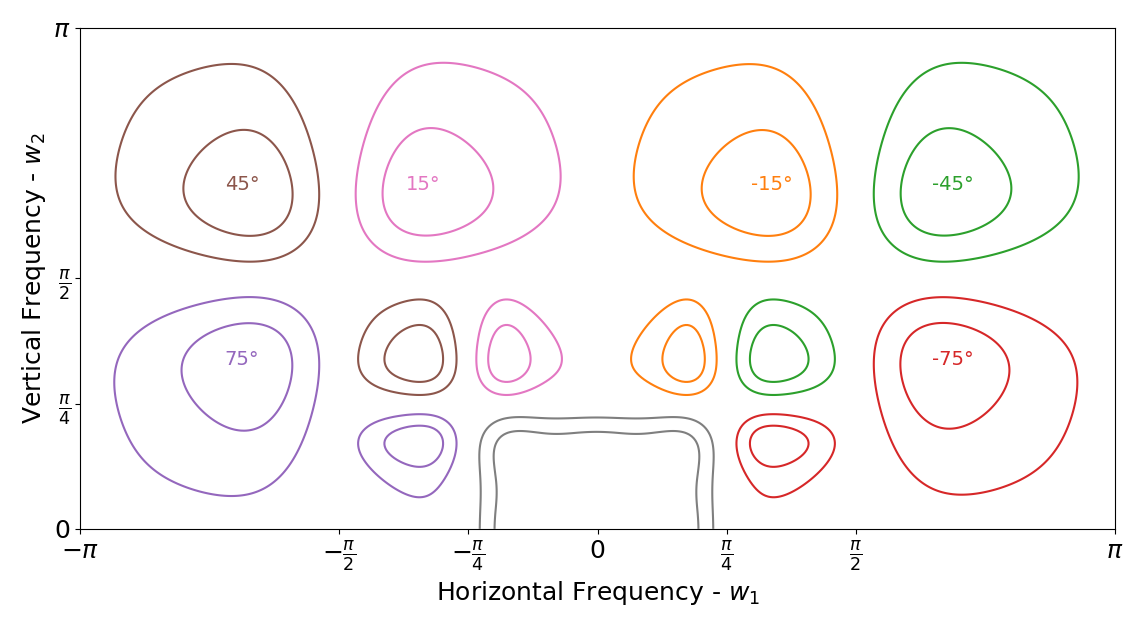
\includegraphics[height=6cm]{\imgpath/subbands.png}
    \label{fig:ch6:dtcwt_bands_freq}
  }
  \hspace{1cm}
%    \newline
  \subfloat[]{%
    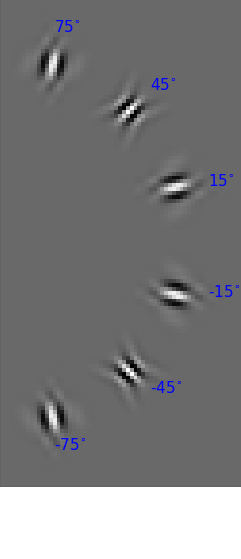
\includegraphics[height=5.7cm]{\imgpath/impulses.png}
    \label{fig:ch6:dtcwt_bands_impulse}
  }
  \mycaption{$\DTCWT$ subbands}{\subref{fig:ch6:dtcwt_bands_freq} -1dB and -3dB contour 
  plots showing the support in the Fourier domain of the 6 subbands of the $\DTCWT$ at scales
  1 and 2, and the scale 2 lowpass. These are the product of the single side
  band filters $P(z)$ and $Q(z)$ from \autoref{thm:ch6:shiftinv}.
  \subref{fig:ch6:dtcwt_bands_impulse} The pixel domain impulse responses for
  the second scale wavelets. The Hilbert pair for each wavelet is the underlying
  sinusoid phase shifted by 90 degrees.}
  \label{fig:ch6:dtcwt_bands}
\end{figure}

\subsubsection{Backpropagation}\label{sec:ch6:dtcwt_update}

We start with the property that for a convolutional block, the
gradient with respect to the input is the gradient with respect to the output
convolved with the time reverse of the filter (proved in \autoref{sec:ch2}).
More formally, if $Y(z) = H(z) X(z)$:
%
\begin{equation}\label{eq:ch6:backprop}
  \Delta X(z) = H(z^{-1}) \Delta Y(z)
\end{equation}
%
where $H(z^{-1})$ is the $Z$-transform of the time/space reverse of $H(z)$,
$\Delta Y(z) \triangleq \dydx{L}{Y}(z)$ is the gradient of the loss with respect
to the output, and $\Delta X(z) \triangleq \dydx{L}{X}(z)$ is the gradient of
the loss with respect to the input. 
If H were complex, the first term in \autoref{eq:ch6:backprop} would be
$\bar{H}(1/\bar{z})$, but as each individual block in the $\DTCWT$ is purely
real, we can use the simpler form $H(z^{-1})$. 

Assume we already have access to the quantity $\Delta Y(z)$ (this is the input
to the backwards pass). \autoref{fig:ch6:bwd_pass} illustrates the
backpropagation procedure.

Let us calculate $\Delta V_r(z)$ and $\Delta V_i(z)$ by backpropagating
$\Delta Y(z)$ through the inverse $\DTCWT$. This is the same as doing the
forward $\DTCWT$ on $\Delta Y(z)$ with the synthesis and analysis filters
swapped and time reversed\footnote{An interesting result is that for orthogonal wavelet
transforms, $S(z^{-1}) = A(z)$, so the backwards pass of an inverse wavelet
transform is equivalent to doing a forward wavelet transform. Similarly, the
backwards pass of the forward transform is equivalent to doing the inverse
transform.}. Then the weight update equations are:
\begin{align}
  \Delta G_r(z) &= \Delta V_r(z) U_r(z^{-1}) + \Delta V_i(z) U_i(z^{-1})  \label{eq:ch6:gr_update}\\
  \Delta G_i(z) &=  -\Delta V_r(z) U_i(z^{-1}) + \Delta V_i(z) U_r(z^{-1})  \label{eq:ch6:gi_update} 
\end{align}
%
The passthrough equations have similar form to \eqref{eq:ch6:dtcwt_fwd}:
\begin{equation}\label{eq:ch6:dtcwt_passthrough}
    \Delta X(z) = \frac{2\Delta Y(z)}{M} \left[G_r(z^{-M})\left( A_r(z)S_r(z) + A_i(z)S_i(z) \right) + \\
       jG_i(z^{-M}) \left(A_r(z)S_i(z) - A_i(z)S_r(z) \right) \right] 
\end{equation}


\subsection{Examples}
\autoref{fig:ch6:examples} show example impulse responses of the $\DTCWT$ gain
layer. For comparison, we also show similar `impulse responses' for a gain layer
done in the DWT domain\footnote{Modifying DWT coefficients causes a loss of the
alias cancellation properties so these are not true impulse response.}. The DWT 
outputs come from three random variables: a $1\x 1$ 
convolutional weight applied to each of the low-high, high-low and high-high
subbands. The $\DTCWT$ outputs come from twelve random variables, again a $1\x
1$ convolutional weight, but now applied to six complex subbands. 
Our experiments have shown that the distribution of the normalized
cross-correlation between 512 of such randomly generated shapes for the DWT matches the
distribution for random vectors with roughly 2.8 degrees of freedom (c.f. 3
random variables in the layer). Similarly for the $\DTCWT$, the distribution of
the normalized cross-correlation matches the distribution for random vectors
with roughtly 11.5 degrees of freedom (c.f. 12 random variables in the layer).
This is particularly reassuring for the $\DTCWT$ as it is showing that there is
still representatitve power despite the redundancy of the transform.

\begin{figure}
  \centering
  \subfloat[]{%
    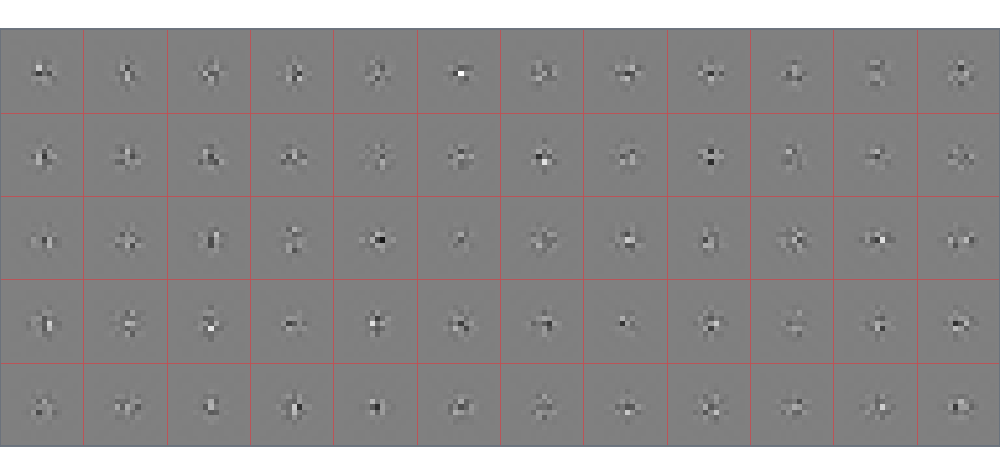
\includegraphics[width=\textwidth]{\imgpath/dtcwt_examples.png}
    \label{fig:ch6:dtcwt_examples}
  }
  \newline
  \subfloat[]{%
  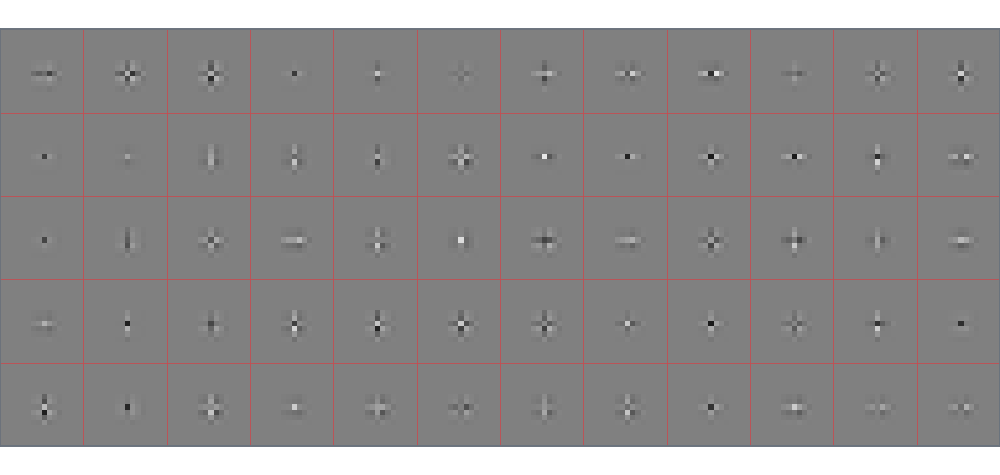
\includegraphics[width=\textwidth]{\imgpath/dwt_examples.png}
    \label{fig:ch6:dwt_examples}
  }
  \mycaption{Example outputs from an impulse input for the proposed gain layers}{
  Example outputs $y = W^{-1}GWx$ for an impulse
  $x$ for the $\DTCWT$ gain layer and for a similarly designed DWT gain layer.
  \subref{fig:ch6:dtcwt_examples} shows the output $y$ for a $\DTCWT$ based
  system. $g_{lp} = 0$ and $g_1$ has spatial size $1\x 1$. The 12 values
  in $g_1$ are independently sampled from a random normal of variance 1.
  The 60 samples come from 60 different random draws of the weights.
  \subref{fig:ch6:dwt_examples}
  shows the outputs $y$ when $x$ is an impulse and $W$ is the DWT with a
  `db2' wavelet family. The strong horizontal and vertical properties of the DWT
  can clearly be seen in comparison to the much freer $\DTCWT$.}
  \label{fig:ch6:examples}
\end{figure}


\subsection{Implementation Details}
Before analyzing its performance, we compare the implementation properties of
our proposed layer to a standard convolutional layer.

\subsubsection{Parameter Memory Cost}\label{sec:ch6:memory}
A standard convolutional layer with $C_l$ input channels, $C_{l+1}$ output channels
and kernel size $k\x k$ has $k^2C_{l}C_{l+1}$ parameters, with $k=3$ or $k=5$
common choices for the spatial size.
\begin{equation}
  \text{\#conv params} = k^2C_lC_{l+1}
\end{equation}

We must choose the spatial sizes of both the lowpass and bandpass
mixing kernels. In our work, we are somewhat limited in how large we would like
to set the bandpass spatial size, as every extra pixel of support requires $2\x
6=12$ extra parameters. For this reason, we almost always set it to have 
support $1\x 1$. The lowpass gains are less costly, and we are free to set them to size
$k_{lp}\x k_{lp}$ (with $k_{lp} = 1,3,5$ in many of our experiments).
%
Further, due to the size of the datasets we test on, we typically limit
ourselves initially to only considering a single scale. If we wish, we can
decompose the input into more scales, resulting in a larger net area of effect.
In particular, it may be useful to do a two scale transform and discard the
first scale coefficients. This does not increase the number of gains to learn,
but changes the position of the bands in the frequency space.

The number of parameters for the gain layer with $k_{lp}=1$ is then:
\begin{equation}
  \text{\#params} = (2\x 6 + 1)C_lC_{l+1} = 13C_lC_{l+1} \label{eq:ch6:memcost2}
\end{equation} 
%
This is slightly larger than the $9C_lC_{l+1}$ parameters used in a
standard $3\x 3$ convolution, but as \autoref{fig:ch6:examples} shows, the
spatial support of the full filter is larger than an equivalent one
parameterized in the filter domain. If $k_{lp}=3$ then we would have $21C_l
C_{l+1}$ parameters, slightly fewer than a $5\x 5$ convolution.

\subsubsection{Activation Memory Cost}\label{sec:ch6:act_memory}
A standard convolutional layer needs to save the activation $x^{(l)}$ to
convolve with the backpropagated gradient $\dydx{L}{y^{(l+1)}}$ on the backwards
pass (to give $\dydx{L}{w^{(l)}}$). For an input with $C_l$ channels of spatial
size $H\x W$, this means
%
\begin{equation}
  \text{\#conv floats} = HWC_l 
\end{equation}

Our layers require us to save the wavelet coefficients $u_{lp}$ and $u_{j,k}$
for updating the $g$ terms as in \eqref{eq:ch6:gr_update} and \eqref{eq:ch6:gi_update}.  
For the $4:1$ redundant $\DTCWT$, this requires:
%
\begin{equation}
  \text{\#$\DTCWT$ floats} = 4HWC_l 
\end{equation}
%
to be saved for the backwards pass.  You can see this difference from the
difference in the block diagrams in \autoref{fig:ch6:block_diagrams}.

Note that a single scale $\DTCWT$ gain layer requires $16/7$ times as many
floats to be saved as compared to the invariant layer of the previous chapter.
The extra cost of this comes from two things. Firstly, we keep the real and
imaginary components for the bandpass (as opposed to only the magnitude),
meaning we need $3HWC_l$ floats, rather than $\frac{3}{2}HWC_l$. Additionally,
the lowpass was downsampled in the previous chapter, requiring only
$\frac{1}{4}HWC_l$, whereas we keep the full sample rate, costing $HWC_l$.

If memory is an issue and the computation of the $\DTCWT$ is very fast, then we
only need to save the $x^{(l)}$ coefficients and can calculate the $u$'s on the
fly during the backwards pass. Note that a two scale $\DTCWT$ gain layer would
still only require $4HWC_l$ floats.

\subsubsection{Computational Cost}\label{sec:ch6:computation}
A standard convolutional layer with kernel size $k\x k$ needs $k^2C_{l+1}$
multiplies per input pixel (of which there are $C_{l}\x H\x W$).

For the $\DTCWT$, the overhead calculations are the same as in
\autoref{sec:ch5:computation}, so we will omit their derivation here. The mixing
is however different, requiring complex convolution for the bandpass
coefficients, and convolution over a higher resolution lowpass. The bandpass has
one quarter spatial resolution at the first scale, but this is offset by the
$4:1$ cost of complex multiplies compared to real multiplies. Again assuming we
have set $J=1$ and $k_{lp} = 1$ then the total cost for the gain layer is:
%
\begin{equation}
  % \frac{7}{4}C_{l+1} + 48 \label{eq:comp}
  \text{\#mults/pixel} = \underbrace{\hphantom{1} \frac{6\x 4}{4}C_{l+1} \hphantom{1}}_{\textrm{bandpass}} +
  \underbrace{\hphantom{1}\vphantom{\frac{6}{4}} C_{l+1} \hphantom{1}}_{\textrm{lowpass}} + 
  \underbrace{\vphantom{\frac{6}{4}} 36}_{\DTCWT} + 
  \underbrace{\vphantom{\frac{6}{4}} 36}_{\DTCWT^{-1}} = \quad 7C_{l+1} + 72 \quad
  \label{eq:ch6:comp_dtcwt}
\end{equation}
which is marginally smaller than a $3\x 3$ convolutional layer.

\subsubsection{Parameter Initialization}
For both layer types we use the Glorot Initialization scheme \cite{glorot_understanding_2010}
with $a=1$: 
%
\begin{equation}
  g_{ij} \drawnfrom U\left[ -\sqrt{\frac{6}{(C_l + C_{l+1})k^2}},\ \sqrt{\frac{6}{(C_l + C_{l+1})k^2}}\
  \right] \label{eq:ch6:glorot}
\end{equation}
where $k$ is the kernel size.

\section{Gain Layer Experiments}\label{sec:ch6:gainlayer_experiments}
Before we explore the possibilities and performance of using a
nonlinearity in the wavelet domain, let us present some experiments and results
for the wavelet gain layer. This is the first objective in
\autoref{sec:ch6:learning}, comparing $G$ to $H$.

\subsection{CNN activation regression}\label{sec:ch6:regression}
\begin{figure}[t]
  \centering
  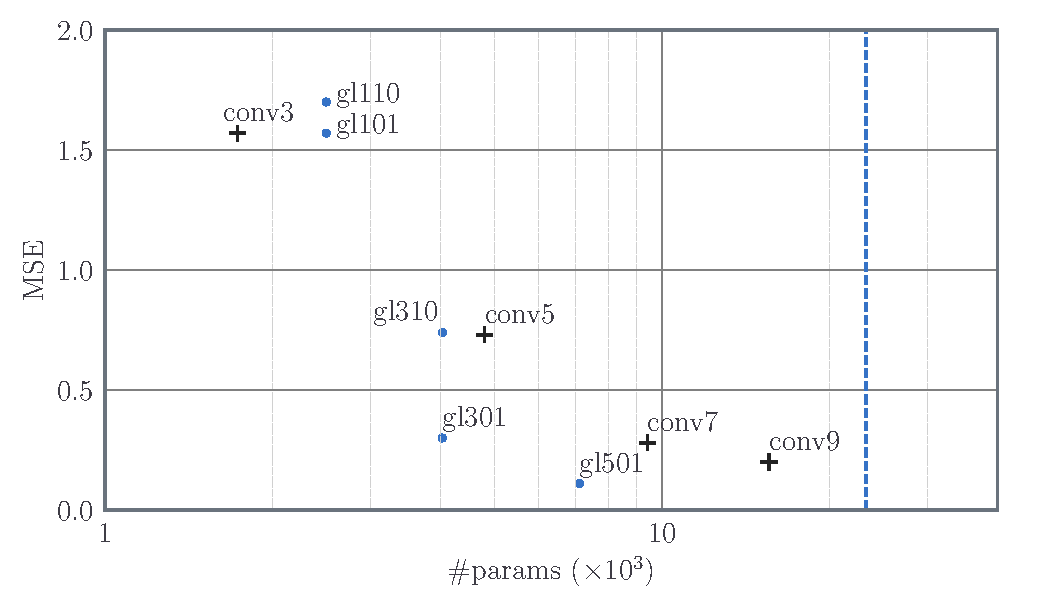
\includegraphics[width=\textwidth]{\imgpath/AlexNet_layer1_regression.pdf}
  \mycaption{Mean Squared Error for Conv and Wavelet Gain Layer Regression with
  AlexNet first layer filters}{After minimization of \eqref{eq:ch6:conv_regression} and
  \eqref{eq:ch6:gain_regression}, this plot shows the final MSE score compared
  to the number of learnable parameters. The original conv layer has spatial
  support $11\x 11$, and the equivalent number of parameters is shown as a blue
  dotted line. The four points labelled `conv$n$' correspond to filters with
  $n\x n$ spatial support. The four points labelled `gl$abc$' correspond to two
  scale gain layers with $a\x a$ support in the lowpass, $b\x b$ spatial support
  in the first scale, and $c\x c$ spatial support in the second scale. The gain
  layer can regress to the AlexNet filters quite capably. In this example, it is
  important to have at least $3\x3$ lowpass support for the gain layer, and the
  second scale coefficients are more important than the first scale.}
  \label{fig:ch6:gainlayer_regression}
\end{figure}
One of the early inspriations for using wavelets in CNNs was the visualizations
of the first layer filters learned in AlexNet. These $11\x 11$ colour filters
(see \autoref{fig:}) look very much like a 2-D oriented wavelet transform.

So how well can the gain layer emulate the action of this layer? How would it
compare to trying to use a reduced size convolutional kernel to learn the 
action of the layer? 

Let us call the action of our target layer $H_0$, our convolutional layer $H$
and our gain layer $G$. Let $\lnorm{H}{2}$, $\lnorm{G}{2}$ be the $\ell_2$ norm
of the weights for each layer. We would like assume that we do not have direct
access to $H_0$ but only the convolved outputs $Y=H_0 X$. Then, we would like to solve:
\begin{align}
  & \argmin_{H}\ (Y - HX)^2 + \frac{\lambda}{2} \lnorm{H}{2}^2 
  \condition{s.t. $h[c, \nn] = 0,\ \forall \nn \notin \mathcal{R}$} \label{eq:ch6:conv_regression}\\
  & \argmin_{G}\ (Y - W^{-1}GWX)^2 + \frac{\lambda}{2} \lnorm{G}{2}^2 
  \condition{s.t. $g_{j,k}[c, \nn] = 0,\ \forall \nn \notin \mathcal{R'}$} \label{eq:ch6:gain_regression}
\end{align}
for some support regions $\mathcal{R},\mathcal{R'}$. E.g. $\mathcal{R}$ could be a $3\x3$ or $5\x5$ 
block, and similarly $\mathcal{R'}$ could define a desired support for each gain in each 
subband. 

\eqref{eq:ch6:conv_regression} and \eqref{eq:ch6:gain_regression} are convex regression
problems, with many possible ways to solve. We are not worried with the
optimization procedure chosen here, but of the final distances $\norm{Y-HX}$
and $\norm{Y-W^{-1}GWx}$ (or equivalently, their squares). We choose to find $H$ and $G$ by 
gradient descent, using the validation set for ImageNet as the data input-output
pair $(X, Y)$. After 3--5 epochs, both $H$ and $G$ typically settle into their
global minimum. Because of the large size of the input filters, we allow for
both a $J=1$ and $J=2$ scale gain layer, but only learn weights at the lowest
frequency bandpass (i.e. for a 2 scale gain layer, we discard the first scale
highpass outputs and only learn $g_2$). 

The resulting MSE are shown in \autoref{fig:ch6:gainlayer_regression}. A label
`gl$ab$' indicates a single scale gain layer with $a\x a$ support in the lowpass
and $b\x b$ support in the highpass; a label `gl$abc$' indicates a two scale
gain layer with $a\x a$ support in the lowpass, $b\x b$ support in the scale 1
highpass and $c\x c$ support in the scale 2 bandpass gains.

This
figure shows several interesting things yet unsurprising things. Firstly, bigger
lowpass support is very helpful -- see the difference between gl101, gl301, and
gl501, 3 instances that only vary in the size of the support of their lowpass
filter $g_{lp}$. Additionally, the second scale coefficients appear more useful
than the first scale -- see the difference between gl310 and gl301, two
instances that have the same number of parameters, but gl310 has $g_1$ with non-zero 
support, and gl301 has $g_2$ with non-zero support.


\subsection{Ablation Studies}
\autoref{fig:ch6:gainlayer_regression} is a useful guide on how the gainlayer
might be placed in a deep CNN. gl110 (a gain layer with a $1\x1$ lowpass kernel
and a $1\x1$ bandpass kernel at the first scale), gl101 (same as gl110 but no
gain at first scale and $1\x 1$ at second scale), and conv3 all achieve similar
MSEs. Additionally gl310, gl301, and conv5 all achieve similar MSEs. 

Most modern CNNs are built with $3\x 3$ kernels, which may not well be the best
use for the gain layer. For this reason, we deviate from the ablation study done
in the previous chapter, and build a shallower network with larger kernel sizes
\footnote{We also include the experiment results for a deeper network with
smaller kernels in \autoref{app:ch6:more_results}.}.

\subsubsection{Large Kernel Ablation}
\begin{table}[ht]
  \renewcommand{\arraystretch}{1.4}
  \centering
  \mycaption{Ablation base architecture}{Reference architecture
  used for experiments on CIFAR-10, CIFAR-100. The activation size rows are offset from the layer description
  rows to convey the input and output shapes. Unlike
  \autoref{tab:ch5:cifar_tiny_arch}, this architecture is shallower and uses
  $5\x 5$ convolutional kernels as a base. $C$ is a hyperparameter that controls
  the network width, we use $C=64$ for our tests. The Tiny ImageNet architecture is
  very similar but with larger activation sizes and one more convolutional
  layer `conv4'.}
  \label{tab:ch6:ablation_arch}
  \makebox[\textwidth]{
    \begin{tabular}{l l l l}
      \toprule
      Activation Size & Reference Arch. && Alternate Arch.\\
      \midrule
      \begin{tabular}{@{}l@{}} % This supresses the space on the left and right
        $3\x 32\x 32$ \\  $C\x 32\x 32$ \\ %$C\x 32\x 32$ \\ 
        $C \x 16\x 16$ \\ $2C\x 16\x 16$ \\ %$2C\x 16\x 16$ \\
        $2C\x 8 \x 8$ \\ $4C\x 8\x 8$ \\ % $4C\x 8\x 8$ \\ 
        $4C\x 1\x 1$ \\ $10$, $100$ 
      \end{tabular} &
      \begin{tabular}{@{}l@{}}
        conv1, $w \in \reals[C\x 3\x 5\x 5]$ \\       
        % batchnorm + relu \\
        pool1, max pool $2\x 2$ \\
        conv2, $w \in \reals[2C\x C\x 5\x 5]$ \\ %, $\F{stride} = 2$\\       
        % batchnorm + relu \\
        pool2, max pool $2\x 2$ \\
        conv3, $w \in \reals[4C\x 2C\x 5\x 5]$\\ % , $\F{stride} = 2$\\       
        % batchnorm + relu \\
        avg, $8\x 8$ average pool \\
        fc1, fully connected 
      \end{tabular} &
      \begin{tabular}{@{}l@{}}
        \emph{or} \\
        \\ 
        \emph{or}\\
        \\ 
        \emph{or}\\
        \\ 
        \\
      \end{tabular} &
      \begin{tabular}{@{}l@{}}
        gain1, $g_{lp} \in \reals[C\x 3\x 3\x 3],\ g_1 \in \complexes[C \x 6\x 3\x 1\x 1]$ \\       
        \\ 
        gain2, $g_{lp} \in \reals[2C\x C\x 3\x 3],\ g_1 \in \complexes[2C \x 6\x C\x 1\x 1]$ \\ %, $\F{stride} = 2$\\       
        \\ 
        gain3, $g_{lp} \in \reals[4C\x 2C\x 3\x 3],\ g_1 \in \complexes[4C \x 6\x 2C\x 1\x 1]$\\ % , $\F{stride} = 2$\\       
        \\ 
        \\
      \end{tabular}\\
      \bottomrule
    \end{tabular}
  }
\end{table}

\renewcommand{\_}{\textscale{.6}{\textunderscore}}

\begin{figure}
  \centering
  \subfloat[CIFAR-10]{%
    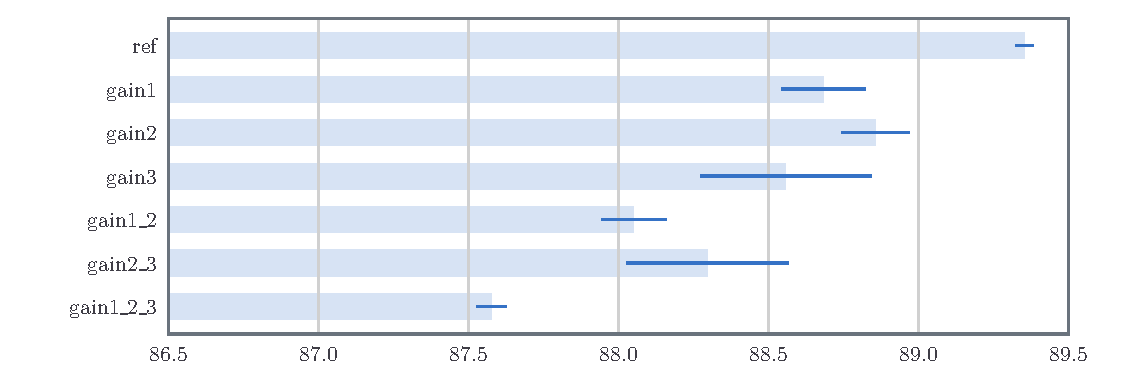
\includegraphics[width=\textwidth]{\imgpath/cifar10_gainlayer_large.pdf}
    \label{fig:ch6:cifar10_gl}
    }\\
  \subfloat[CIFAR-100]{%
    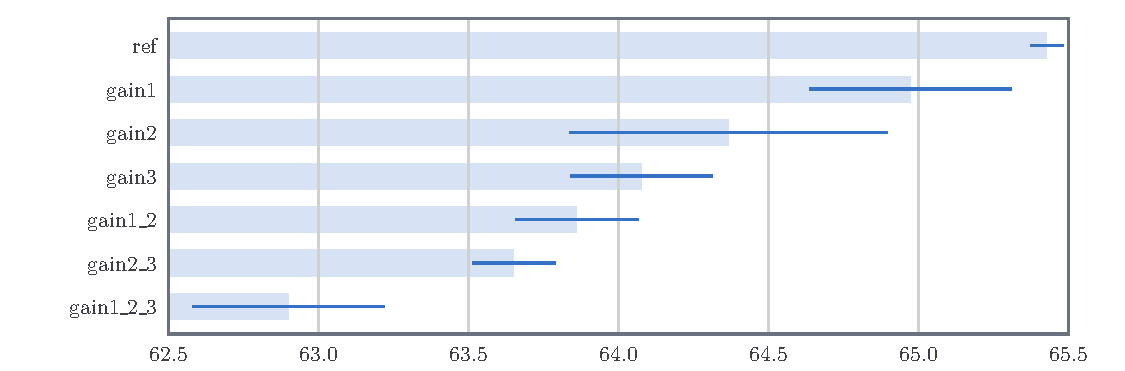
\includegraphics[width=\textwidth]{\imgpath/cifar100_gainlayer_large.pdf}
    \label{fig:ch6:cifar100_gl}
  }\\
  \subfloat[Tiny ImageNet]{%
    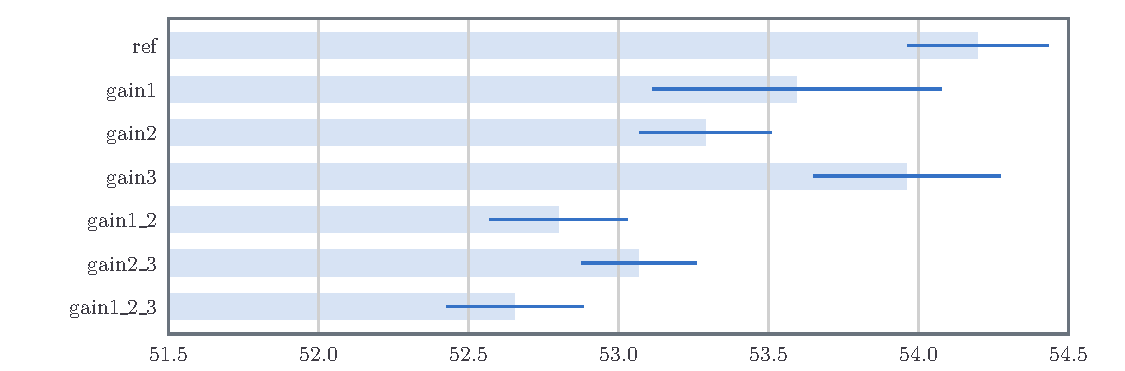
\includegraphics[width=\textwidth]{\imgpath/ti_gainlayer_large.pdf}
    \label{fig:ch6:ti_gl}
  }
  \mycaption{Large kernel ablation results CIFAR and Tiny ImageNet}{Results
  showing the accuracies obtained by swapping combinations of the three conv
  layers in the reference architecture from \autoref{tab:ch6:ablation_arch} with
  gain layers. Results shown are averages of 3 runs with the standard deviations
  shown as dark blue lines. These results show that changing a convolutional
  layer for a gain layer is possible, but comes with a small accuracy cost which 
  compounds as more layers are swapped.}
  \label{fig:ch6:gl_results}
\end{figure}

In this experiment, we build a 3 layer
CNN with $5\x 5$ convolutional kernels, described in \autoref{tab:ch6:ablation_arch}.
To help differentiate with the small kernel network introudeced in the 
ablation study of the previous chapter, we have labelled the convolutions here
`conv1', `conv2' and `conv3' (as opposed to `convA', `convB', `convC',
\ldots).

We then test the difference in accuracy achieved by replacing each of the three
convolution layers with gl310\footnote{Although the gain layers with no gain in
the first scale and gain in the second scale performed better than those with
gain gl310 and gl510 in \autoref{sec:ch6:regression}, we saw them perform
consinstently worse in the following ablation studies. For ease of presentation,
we have shown only the results from the single scale gain layer.}. 
On the two CIFAR datasets, we train for 120 epochs, decaying learning rate by a
factor of 0.2 at 60, 80 and 100 epochs, and for the Tiny ImageNet dataset, we
train for 45 epochs, decaying learning rate at 18, 30 and 40 epochs. The
experiment code is available at \cite{}.

The results of various swaps for our three datasets are shown in
\autoref{fig:ch6:gl_results}.
Note that as before, swapping `conv1' with a gain layer is marked by `gain1',
and swapping the first two conv layers with two gain layers is marked by
`gain1\_2' and so forth.  

The results are not too promising. Across all three datasets, changing a
convolutional layer for a gain layer of similar number of parameters
results in a small decrease in accuracy at all depths, and the more layers
swapped out the more this degradation compounds.


\subsection{Network Analysis}
It is nonetheless interesting to see that a network with only gain layers
(`gain1\_2\_3') can get accuracies within a couple of percentage points of a
purely convolutional architecture. 

In this section, we look at some of the properties of the `gain1\_2\_3' for
CIFAR-100 and compare them to the reference architecture.

\subsubsection{Bandpass Coefficients}
When analyzing the `gain1\_2\_3' architecture, the most noticeable thing is the
distribution of the bandpass gain magnitudes. \autoref{fig:ch6:bp_dists} shows
these for the second gain layer, gain2. Of the $64\x 128=8192$ complex
coefficients most have very small magnitude, in particular the diagonal wavelet
gains. This raises an interesting question -- how many of these coefficients are
important for classification? What if we were to apply a hard thresholding
scheme to the weights, would setting some of these values to 0 impact the
entire network accuracy? 

We measure the dropoff in accuracy when a hard threshold $t$ is applied to the 
bandpass gains $g_1$ for the three gain layers of `gain1\_2\_3'. The resulting sparsity
of each layer and the network performance is shown in \autoref{fig:ch6:threshs}.
This figure shows that despite the high cost of the bandpass gains --
$12C_{l}C_{l+1}$ for a $1\x1$ gain, very few of these need to be nonzero.

\begin{figure}
  \centering
  \vspace{-0.5cm}
  \subfloat[Bandpass Magnitude Distributions]{
    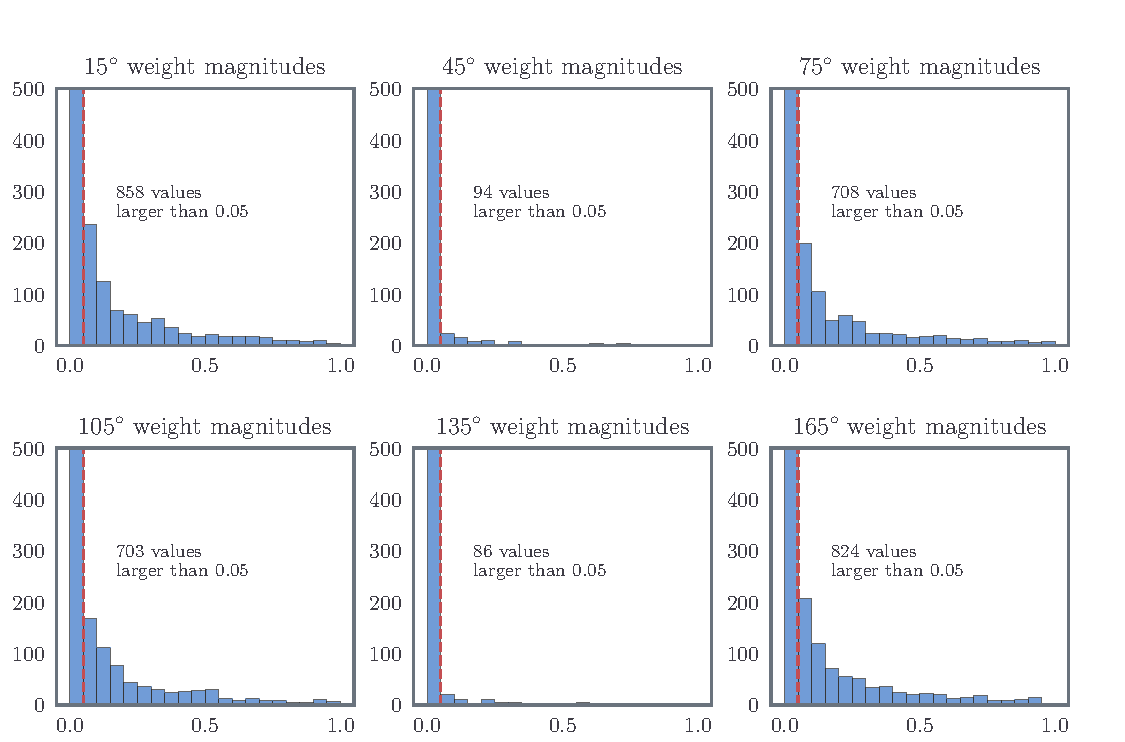
\includegraphics[width=.9\textwidth]{\imgpath/complex_mag_dists.pdf}
    \label{fig:ch6:bp_dists}
    }\\\vspace{-0.3cm}
  \subfloat[Accuracy Dropoff from Thresholding]{
    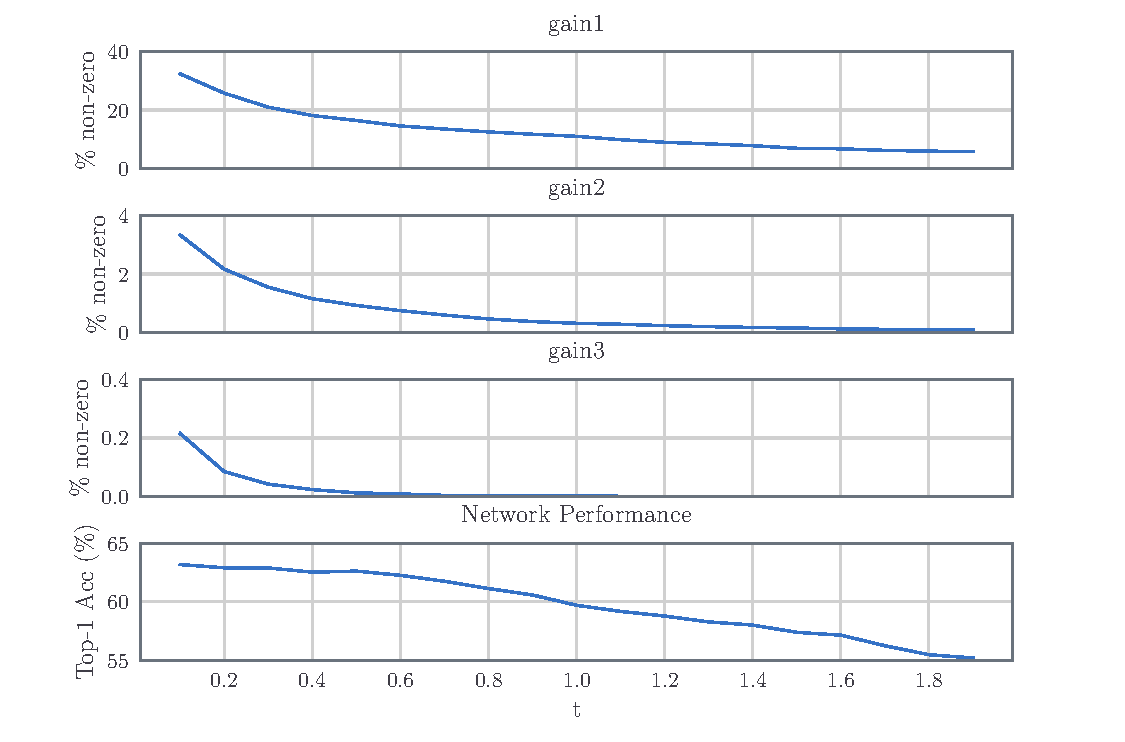
\includegraphics[width=\textwidth]{\imgpath/cifar100_gainlayer_threshs.pdf}
    \label{fig:ch6:threshs}
    }
    % \mycaption{}{}
    \mycaption{Bandpass Gain Properties}{\subref{fig:ch6:bp_dists} shows the
    distribution of the magnitudes for bandpass coefficients for the second
    layer (gain2). Each orientation has $128\x 64=8192$ complex weights, most of
    which are close to or near 0. The $45\degs$ and $135\degs$ weights have many 
    fewer large coefficients. \subref{fig:ch6:threshs} shows the increase in
    sparsity and dropoff in classification accuracy when the weights are
    hard-thresholded with value $t$ (same threshold applied to all 3 layers).
    For a threshold value of $t=0.4$, 80\% of the weights in gain1 are 0, 99\%
    of the weights in gain2 are 0, 99.98\% of the weights in gain3 are 0 and
    classification accuracy is 0.5\% lower than the non-thresholded accuracy.}
  \label{fig:ch6:bp_info}
\end{figure}

\subsubsection{DeConvolution and Filter Sensitivity}

\section{Wavelet Based Nonliearities}
Returning to the goals from \autoref{sec:ch6:learning}, the experiments from the
previous section have shown that while it is possible to use a wavelet gain
layer ($G$) in place of a convolutional layer ($H$), this may come with a small
performance penalty. Ignoring this effect for the moment, in this section, we
continue with our investigations into learning in the wavelet domain. In
particular, is it possible to replace a pixel domain nonlinearity $\sigma$ with
a wavelet based one $\sigma_w$?

But what sensible nonlinearity to use? Two particular options are good initial
candidates:
\begin{enumerate}
  \item The ReLU: this is a mainstay of most modern neural networks and has
    proved invaluable in the pixel domain. Perhaps its sparsifying properties
    will work well on wavelet coefficients too. 
  \item Thresholding: a technique commonly applied to wavelet
    coefficients for denoising and compression. Many proponents of compressed
    sensing and dictionary learning even like to compare soft thresholding to a
    two sided ReLU \cite{papyan_theoretical_2018, papyan_convolutional_2016}.
\end{enumerate}

In this section we will look at each, see if they add to the gain
layer, and see if they open the possibility of having multiple layers in the
wavelet domain. 

\subsection{ReLUs in the Wavelet Domain}
Applying the ReLU to the real lowpass coefficients is not difficult, but it does
not generalize so easily to complex coefficients. The simplest option is to apply
it independently to the real and imaginary coefficients, effectively only
selecting one quadrant of the complex plane:
\begin{align}
  u_{lp} &= \F{max}(0,\ v_{lp}) \\
  u_{j} &= \F{max}(0,\ \real{v_{j}}) + j\F{max}(0,\ \imag{v_j}) \label{eq:ch6:relu_bp}
\end{align}

Another option is to apply it to the magnitude of the bandpass coefficients. Of
course these are all strictly positive so the ReLU on its own would not do
anything. However, they can be arbitrarily scaled and shifted by using a batch
normalization layer. Then the magnitude could shift to (invalid) negative
values, which can then be rectified by the ReLU. %
\begin{align}
  \theta_j &= \arctan \left(\frac{\imag{v_j}}{\real{v_{j}}} \right) \\
  r_j &= \sqrt{\real{v_j}^2 + \imag{v_j}^2} \\
  r_j' &= \max (0,\ BN(r_j)) = \max(0,\ \gamma \frac{r_j-\mu_r}{\sigma_r} + \beta) \label{eq:ch6:magrelu_bp}\\
  u_j &= r_j' e^{j\theta_j}
\end{align}
This also works nicely on the lowpass coefficients:
\begin{equation}
  u_{lp} = \F{max}(0,\ BN(v_{lp})) \label{eq:ch6:bnrelu_lp}
\end{equation}
%
\subsection{Thresholding}
The soft and hard thresholding operators for a threshold $t>0$ are defined as:
\begin{align}
  \mathcal{H}(x, t) &= \indic(|x| > t)x \\
  \mathcal{S}(x, t) &= \sgn(x)\max(0,\ |x| - t)  \\
                    &= \frac{x}{|x|}\max(0,\ |x|-t) \label{eq:ch6:relu_st}
\end{align}
Note that \eqref{eq:ch6:relu_st} is very similar to \eqref{eq:ch6:magrelu_bp} as $r_j \geq 0$. We
can rewrite \eqref{eq:ch6:magrelu_bp} by taking the strictly positive terms
$\gamma$, $\sigma$ outside of the $\max$ operator:
\begin{align}
  r_j' &= \max(0, \gamma \frac{r_j-\mu}{\sigma} + \beta) \\
       &= \frac{\gamma}{\sigma_r}\max\left(0, r_j - \mu_r + \frac{\sigma_r\beta}{\gamma}\right) 
\end{align}
then if $t' = \mu_r - \frac{\sigma_r\beta}{\gamma} > 0$, doing batch
normalization followed by a ReLU on the magnitude of the coefficients is the
same as soft shrinkage with threshold $t'$, scaled by a factor
$\frac{\gamma}{\sigma_r}$.  The same analogy does not apply to the lowpass
coefficients, as $v_{lp}$ is not strictly positive. 

To get strict soft or hard thresholding for the low and bandpass coefficients,
we have the option of learning the threshold $t$ or setting it to achieve a
desired sparsity level. In early experiments we found that any 
learnt threshold $t$ quickly goes to 0, turning off the thresholding. We can
force some sparsity level however by keeping a track of the moments of the activations with an
exponential moving average, and finding quantiles by matching the distribution of
the activations. For the bandpass coefficients, the activations very nearly
follow an exponential distribution. The lowpass coefficients are a bit more
varied, following a generalized Gaussian distribution (GGD) with shape parameter
$\beta$ ranging from 0.6 for the earlier layers to ~1.5 for deepr layers.

\subsection{Non-Linearity Experiments}
\begin{algorithm}[t]
  \caption{The \emph{wave layer} pseudocode}\label{alg:ch6:wavelayer}
\begin{algorithmic}[1]
  \Procedure{WaveLayer}{$x$}
  \State $u_{lp},\ u_{1} \gets \DTCWT(x, \mbox{nlevels}=1) $ 
  \State $v_{lp},\ v_{1} \gets G(u_{lp},\ u_{1}) $ \Comment{the normal wave gain layer}
  \State $w_{lp} \gets \sigma_{lp}(v_{lp})$ \Comment{lowpass nonlinearity}
  \State $w_{1} \gets \sigma_{bp}(v_{1})$ \Comment{bandpass nonlinearity}
  \State $y \gets \DTCWT^{-1}(w_{lp},\ w_{1})$
  \State $x \gets \sigma_{pixel}(y)$ \Comment{pixel nonlinearity}
  \State \textbf{return} $x$
\EndProcedure
\end{algorithmic}
\end{algorithm}
Taking the same `gain1\_2\_3' architecture used for CIFAR-100, we expand the
\emph{wave gain layer} into one bigger layer
dubbed the \emph{wave layer}, described in \autoref{alg:ch6:wavelayer}. In the wave
layer, there are we have 3 different nonliearities: the pixel, the lowpass 
and the bandpass nonlinearity.

For these experiments, we test over a grid of possible options for these three
functions:
\begin{table}[h!]
  \centering
\begin{tabular}{l l l l l l l}
  \toprule
  Nonlinearity & \hphantom{abc} & \multicolumn{5}{c}{Values} \\
  \midrule
  Pixel && None & BN+ReLU \\
  Lowpass && None & ReLU & BN+ReLU & $\mathcal{S}$ & $\mathcal{H}$  \\
  Bandpass && None & ReLU & BN+MagReLU & $\mathcal{S}$ & $\mathcal{H}$ 
  \\\bottomrule
\end{tabular}
\end{table}

Where:
\begin{itemize}
  \item `None' means no nonlinearity -- $\sigma(x) = x$.
  \item `BN+ReLU' is batch normalization and ReLU (applies only to real valued
    activations) e.g. \eqref{eq:ch6:bnrelu_lp}.
  \item `ReLU' is a ReLU without batch normalization. Can be applied to the real
    and imaginary parts of a complex activation independently i.e.
    \eqref{eq:ch6:relu_bp}.
  \item `BN+MagReLU' applies batch normalization to the magnitude of complex
    coefficients and then makes them strictly positive with a ReLU. See
    \eqref{eq:ch6:magrelu_bp}.
  \item $\mathcal{S}$ and $\mathcal{H}$ are the soft and hard thresholding
    operators applied to the magnitudes of coefficients. We choose a
    conservative sparsity level of 0.2 (20\% of coefficients set to 0) for these
    thresholds. A full grid search over
    sparsity levels would be beneficial, but setting it low initially allows us
    to test its plausibility as a nonlinearity.
\end{itemize}

As the pixel nonliearity has only two options, the results are best displayed as
a pair of tables, firstly for no nonlinearity and secondly for the
the standard batch normalization and ReLU. See
\autoref{tab:ch6:nonlinearities} for these two tables. 

Digesting this information gives us some useful insights: 
\begin{enumerate}
  \item It is possible to improve on the gainlayer from the previous experiments
    (top left entry of the second table) with the right nonlinearities.
  \item Looking at the fourth and fifth rows/columns of both tables, soft and
    hard thresholding for both the lowpass and bandpass coefficients does not perform as
    well as ReLUs (and sometimes worse than no nonlinearity) even with a low
    sparsity level. We saw this performance worsen as the sparsity level
    increased.
  \item Doing a ReLU on the real and imaginary parts of the bandpass
    coefficients independently (the second row of both tables) almost always
    performs worse than having no nonlinearity (first row of both tables).
  \item The best combination is to have batch normalization and a ReLU applied
    to the magnitudes of the bandpass coefficients and batch norm and a ReLU
    applied to either the lowpass or pixel coefficients. 
\end{enumerate}

The best accuracy score of $65.5\%$ is now $0.4\%$ lower than the fully
convolutional architecture, however this network has slightly fewer parameters.

% \begin{table}[t]
  % \centering
  % \renewcommand{\arraystretch}{1.2}
% \begin{tabular}{ll| l l l l l}
  % && \multicolumn{5}{c}{$\sigma_{bp}$} \\
  % && None & ReLU & BN+MagReLU & $\mathcal{S}$ & $\mathcal{H}$ \\
  % \midrule
  % \multirow{5}{*}{$\sigma_{lp}$} & None & \\
                          % &ReLU & \\
                           % &BN+ReLU & \\
                           % &$\mathcal{S}$ & \\
                           % & $\mathcal{H}$ & \\ 
% \end{tabular}
% \end{table}

\begin{table}[t]
  \renewcommand{\arraystretch}{1.2}
  \small
  \centering
  \def \mywidth {1.4cm}
  \mycaption{Different Nonlinearities in the Gain Layer}{Top-1 Accuracies for
  `gain1\_2\_3' network trained on CIFAR-100 using different wavelet and pixel nonlinearities.
  The rows of the table correspond to different bandpass nonlinearities and the
  columns correspond to different lowpass nonlinearities.
  $\sigma_{pixel}=\sigma_{lp}=\sigma_{bp}=\text{None}$ is a linear system (with
  max pooling). $\sigma_{pixel}=\F{ReLU},\ \sigma_{lp}=\sigma_{bp}=\text{None}$
  is the system used in earlier experiments which is linear in the wavelet
  domain and has a nonlinearity in the pixel domain. Results are averages over
  3 runs.}
  \label{tab:ch6:nonlinearities}
  \subfloat[$\sigma_{pixel} = \text{None}$]{%
  \centering
  \makebox[\textwidth][c]{
  \begin{tabular}{l |p{\mywidth} p{\mywidth} p{\mywidth} p{\mywidth} p{\mywidth} }
      \toprule
      \diagbox[width=3cm]{$\sigma_{bp}$}{$\sigma_{lp}$}& None & ReLU & BN+ReLU & $\mathcal{S}$ & $\mathcal{H}$ \\
      \hline
      None & 45.0 & 63.1 & 64.4 & 54.1 & 42.5 \\
      ReLU & 42.6 & 62.4 & 63.9 & 54.4 & 41.8\\
      BN+MagReLU & 48.5 & 65.5 & 65.0 & X & X\\
      $\mathcal{S}$ & X & X & X & X & X \\
      $\mathcal{H}$ & 41.3 & 60.7 & X & 52.0 & 40.6\\ 
      \bottomrule
    \end{tabular}
  }}\newline
  \subfloat[$\sigma_{pixel} = \F{BN+ReLU}$]{
  \centering
  \makebox[\textwidth][c]{
  \begin{tabular}{l |p{\mywidth} p{\mywidth} p{\mywidth} p{\mywidth} p{\mywidth} }
      \toprule
      \diagbox[width=3cm]{$\sigma_{bp}$}{$\sigma_{lp}$}& None & ReLU & BN+ReLU & $\mathcal{S}$ & $ \mathcal{H}$ \\
      \hline
      None & 62.8 & 62.0 & 65.0 & 62.8 & 62.9 \\
      ReLU & 62.8 & 61.4 & 64.6 & 61.6 & 61.8 \\
      BN+MagReLU & 64.5 & 63.1 & 64.5 \\
      $\mathcal{S}$ \\
      $\mathcal{H}$ & 59.7 & 58.7 & & 59.6 & 59.7\\ 
      \bottomrule
    \end{tabular}
    }}
\end{table}

\section{Conclusion}
In this chapter we have presented the novel idea of learning filters by taking
activations into the wavelet domain. In the wavelet domain then we can apply
the proposed gain layer $G$ instead of a pixel wise convolution, and can apply
wavelet based nonlinearities $\sigma_w$. We have considered the possible
challenges this proposes and described how a multirate system can learn through
backpropagation. 
%We ultimately hope that learning in both the wavelet and pixel
%space will have many advantages. 
Our experiments have been promising but not convincing. We have shown that our layer can learn in an
end-to-end system, achieving similar accuracies on CIFAR-10, CIFAR-100 and Tiny
ImageNet to the same system with convolutional layers instead. This is a good
start and shows the plausibility of the wavelet gain layer, but we have not yet
seen a benefit to learning in the wavelet space. 

We have searched for good candidates for wavelet nonlinearities, and saw that
using Batch Normalization followed by a ReLU on the lowpass coefficients, and
Batch Normalization and a ReLU on the magnitudes of the bandpass coefficients
improved the performance of the gain layer considerably, but still not enough to
warrant 
